%!TEX root = ../thesis.tex
%*******************************************************************************
%********************************* Seventh Chapter *****************************
%*******************************************************************************
\cleardoublepage
\chapter{Reliability and robustness analysis of an offshore wind turbine subject to fatigue}
\label{chpt:7}
%*******************************************************************************
\hfill
\localtableofcontents
\newpage

%============================================================%
%============================================================%
\section{Introduction}
%============================================================%
%============================================================%
One of the main goals of this work is to evaluate the reliability of an OWT's monopile foundation w.r.t. fatigue solicitations. 
Let us recall the approach to assess fatigue damage over the structure's lifetime (see \citealp[Appendix H]{iec_2019}). 
First, the lifetime before decommissioning time $t_{\mathrm{d}}\in\R_+$ forms the interval $T=[0, t_{\mathrm{d}}]$, which can be used to define a probability space $(T, \iB(T), \iU(T)=\lambda / t_{\mathrm{d}})$. 
Then, for all $t\in T$ and assuming the probability space $(\Omega, \iA, \P)$, the random vector of the environmental conditions $\bX(t, \cdot)$ is a measurable function on $(\Omega, \iA) \rightarrow (\R^d, \iB(\R^d))$.  
Therefore, one can define the product probability space $(T\times\Omega, \, \iB(T) \otimes \iA, \, \iU(T) \otimes \P)$ and the random vector $\bX$, which is a measurable function on $(T \times \Omega, \, \iB(T) \otimes \iA) \rightarrow (\R^d, \iB(\R^d))$.  
For a realization of $\bX$, denoted by $\bX\left(t^{(i)}, \omega^{(r)}\right)$, and a given set of parameters $\bz=\left(k_{\mathrm{soil}}, \theta_{\mathrm{yaw}}, \varepsilon\right)$ related to the system (defined in Table~\ref{tab:sys_variables}), one can perform a 10-minute Turbsim-DIEGO simulation (see Subsection~\ref{sec:235}) to obtain the corresponding cumulative damage:
\begin{equation}
    d_{\mathrm{c}}^{10\mathrm{min}}\left(\bX\left(t^{(i)}, \omega^{(r)}\right)\,|\,\bZ=\bz\right). 
\end{equation}
In practice, $T$ is often discretized into $N_T \in \N$ 10-minute intervals $\left\{t^{(i)}\right\}_{i=1}^{N_T}$ \citep[Appendix H]{iec_2019}. 
The 10-minute duration results from the typical wind energy distribution (see \fig{fig:wind_psd}), presenting a ``short-term'' behavior (for turbulent wind with a return period below 10 minutes) and ``long-term'' behavior (otherwise, which is defined in Table~\ref{tab:envi_variables}).
To cumulate the damage over the lifetime, one can write the sum of 10-minute damages, each averaged over $n_{\mathrm{rep}} \in \N$ pseudo-random seed repetitions: 
\begin{subequations}
    \begin{align}
        D(\bz) &= N_T \, \E\left[d_{\mathrm{c}}^{10\mathrm{min}}(\bX\,|\,\bZ=\bz)\right]\\
             & \approx N_T \frac{1}{N_T \, n_{\mathrm{rep}}} \, \sum_{i=1}^{N_T} \sum_{r=1}^{n_{\mathrm{rep}}} d_{\mathrm{c}}^{10\mathrm{min}}\left(\bX\left(t^{(i)}, \omega^{(r)}\right)\,|\,\bZ=\bz\right).
             \label{eq:expected_damage}
    \end{align}
\end{subequations}

In Chapter~\ref{chpt:4}, KH was proposed as a method for given-data subsampling to propagate the uncertain environmental conditions on Teesside's OWT model. 
This method showed equivalent performances to QMC for estimating the lifetime damage in \eq{eq:expected_damage}, while being more flexible than QMC. 
In the linear cumulative damage model typically used by the community (Miner's rule), a damage value higher than one leads to ruin of the structure by convention. 
The present chapter assesses the probability of such a rare event, considering both the environmental uncertainties (aggregated according to \eq{eq:expected_damage}) and the uncertainties related to the system itself (described by the random vector $\bZ \in \iD_\bZ$ with joint PDF $f_\bZ$). 
Assuming that the critical damage $D_{\mathrm{cr}}$ is a random variable centered around one (equivalent to a ``resistance'' variable in the well-known ``resistance-solicitation'' paradigm in reliability analysis \citealp{lemaire_2009}), this failure probability is written as:
\begin{equation}
    \pf = \int_{\iD_\bZ} \1_{\{D(\bz) \geq D_{\mathrm{cr}}\}} \, f_\bZ(\bz) \, \dd z \,.
    \label{eq:owt_pf}
\end{equation}

Less information is available to define the probabilistic model of the system uncertainties than the environmental ones. 
Therefore, the robustness analysis of the failure probability w.r.t. the probabilistic model $\bZ$ should be studied. 
To do so, a perturbation-based approach using the \textit{perturbed-law based sensitivity indices} (PLI), originally introduced by \citep{lemaitre_2015_PLI}, is used in this chapter.   
However, the reliability and robustness analysis requires a number of evaluations of the Turbsim-DIEGO simulator $D(\cdot)$ that would be prohibitive without the use of surrogate models. 

The present chapter is structured as follows: 
Section~\ref{sec:owt_surrogate} presents the construction of a surrogate model of $D(\cdot)$,
then Subsection~\ref{sec:owt_ra} analyses the reliability of the monopile foundation of Teesside's turbine for a nominal distribution of $\bZ$, 
and finally Subsection~\ref{sec:owt_robustness} proposes a robustness analysis of $\pf$ by perturbing the laws of both $\bZ$ and $D_{\mathrm{cr}}$.

%============================================================%
%============================================================%
\section{Surrogate modeling for reliability analysis}\label{sec:owt_surrogate}
%============================================================%
%============================================================%
The prohibitive computational cost of the function $D(\cdot)$ requires fitting a surrogate model.  
This section presents the specific high-performance computer (HPC) wrapper developed for this application and how it is used to build a learning set for a GP regression model. 

%============================================================%
\subsection{High-performance computer evaluation}
%============================================================%
The wrapper of the numerical chain including Turbsim and Diego (illustrated in \fig{fig:owt_chained_model}) for reliability analysis has a nested double loop structure. 
The outer loop pilots the realizations of $\bZ$ while the inner loop concerns the environmental conditions and their repetitions for $n_{\mathrm{rep}}$ different pseudo-random seeds. 
At this stage, the goal is to approximate $D(\cdot)$ for any value of $\bz = (k_{\mathrm{soil}}, \theta_{\mathrm{yaw}}, \varepsilon=1)$, since $\varepsilon$ is a coefficient applied to the damage as post-processing (see Subsection~\ref{sec:probabilistic_sn}). 
Using a KH design to explore the environmental conditions as discussed in Chapter~\ref{chpt:4}, this approximation is written as: 
\begin{equation}
    D(\bz) \approx D^{\mathrm{KH}}(\bz) = N_T \frac{1}{n_\bX n_{\mathrm{rep}}} \sum_{i=1}^{n_\bX} \sum_{r=1}^{n_{\mathrm{rep}}} d_{\mathrm{c}}^{10\mathrm{min}}\left(\bx^{(i)}, \omega^{(r)} \,|\, \bZ = \bz = (k_{\mathrm{soil}}, \theta_{\mathrm{yaw}}, \varepsilon=1)\right)\, ,
    \label{eq:hpc_cumulated_damage}
\end{equation}
where a KH design with size $n_\bX \in \N$ is denoted by $\left\{\bx^{(i)}\right\}_{i=1}^{n_\bX}$. 
According to the convergence results obtained in Chapter~\ref{chpt:4}, the KH size is fixed at $n_\bX=200$ and the repetitions at $n_{\mathrm{rep}}=11$, which implies a total of $2200$ Turbsim-DIEGO simulations per evaluation of the function $D^{\mathrm{KH}}(\cdot)$. 
In this setup, the CRONOS HPC from EDF R\&D allows us to simultaneously perform those 2200 simulations in parallel. 
The random variable associated with the S-N curve uncertainty is introduced later as a product factor of \eq{eq:hpc_cumulated_damage}. 
Note that the cumulative damage studied is actually the maximum value of $D^{\mathrm{KH}}(\cdot)$ over the discretized azimuth angles (illustrated in \fig{fig:wind_wave_roses}), at the mudline level. 


%============================================================%
\subsection{Design of experiments}
%============================================================%
To build a learning set, a space-filling design of experiments is created on the joint domain of $(K_{\mathrm{soil}}, \Theta_{\mathrm{yaw}})$. 
This design was first composed of 30 points generated by a Halton sequence (illustrated in \fig{fig:initial_doe}.a) which was the most space-filling sequential method (compared to other QMC sequences and KH). 
Its evaluation and analysis showed that the highest damage values are the result of high absolute values of $\Theta_{\mathrm{yaw}}$ or low values of $K_{\mathrm{soil}}$. 
Therefore, the design was completed in a second phase by 20 points targeting these areas by applying kernel herding to a subdomain defined a priori (see the candidate set represented by the gray points in \fig{fig:initial_doe}.b). 
Finally, the learning set is the union of the two complementary designs, later referred to as the ``mixed design'' (see \fig{fig:initial_doe}.b). 
This mixed design, denoted by $\bZ_{n_\bZ}$, has a size of $n_\bZ=50$ points, which represents over $10^5$ Turbsim-DIEGO simulations (each requiring around 45 minutes of CPU time).
\fig{fig:evaluated_doe} shows the lifetime cumulated damage evaluated on the mixed design (with normalized values corresponding to the color scale). 

%\elias{Comment on the fact that it's not symmetric}. 
%\elias{the damage values are obtained for a nominal S-N curve defined in xxxx for Teesside's model defined in Chapter 4}

\footnotetext{text}


\begin{figure}
    \centering
    \begin{subfigure}{0.48\linewidth}
        \vskip -30pt
        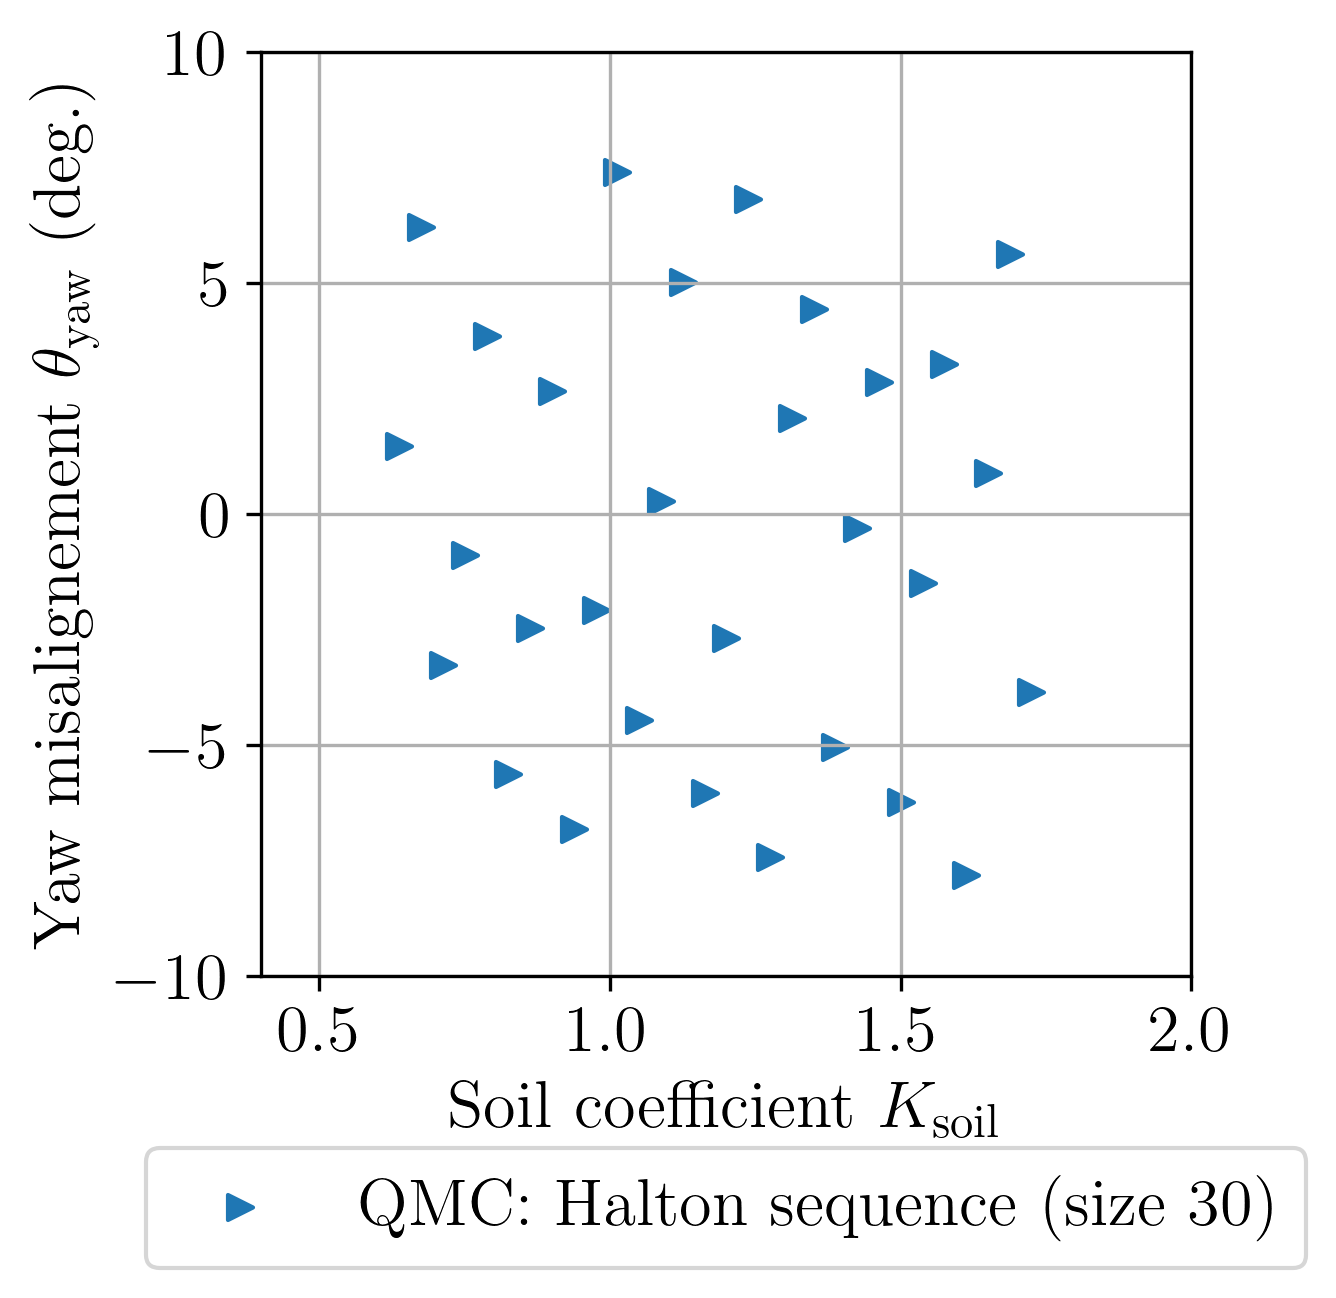
\includegraphics[width=\linewidth]{./part3/figures/OWT/initial_halton.png}
        \caption{Halton sequence.}
    \end{subfigure}
    \begin{subfigure}{0.48\linewidth}
        %\vskip 0pt
        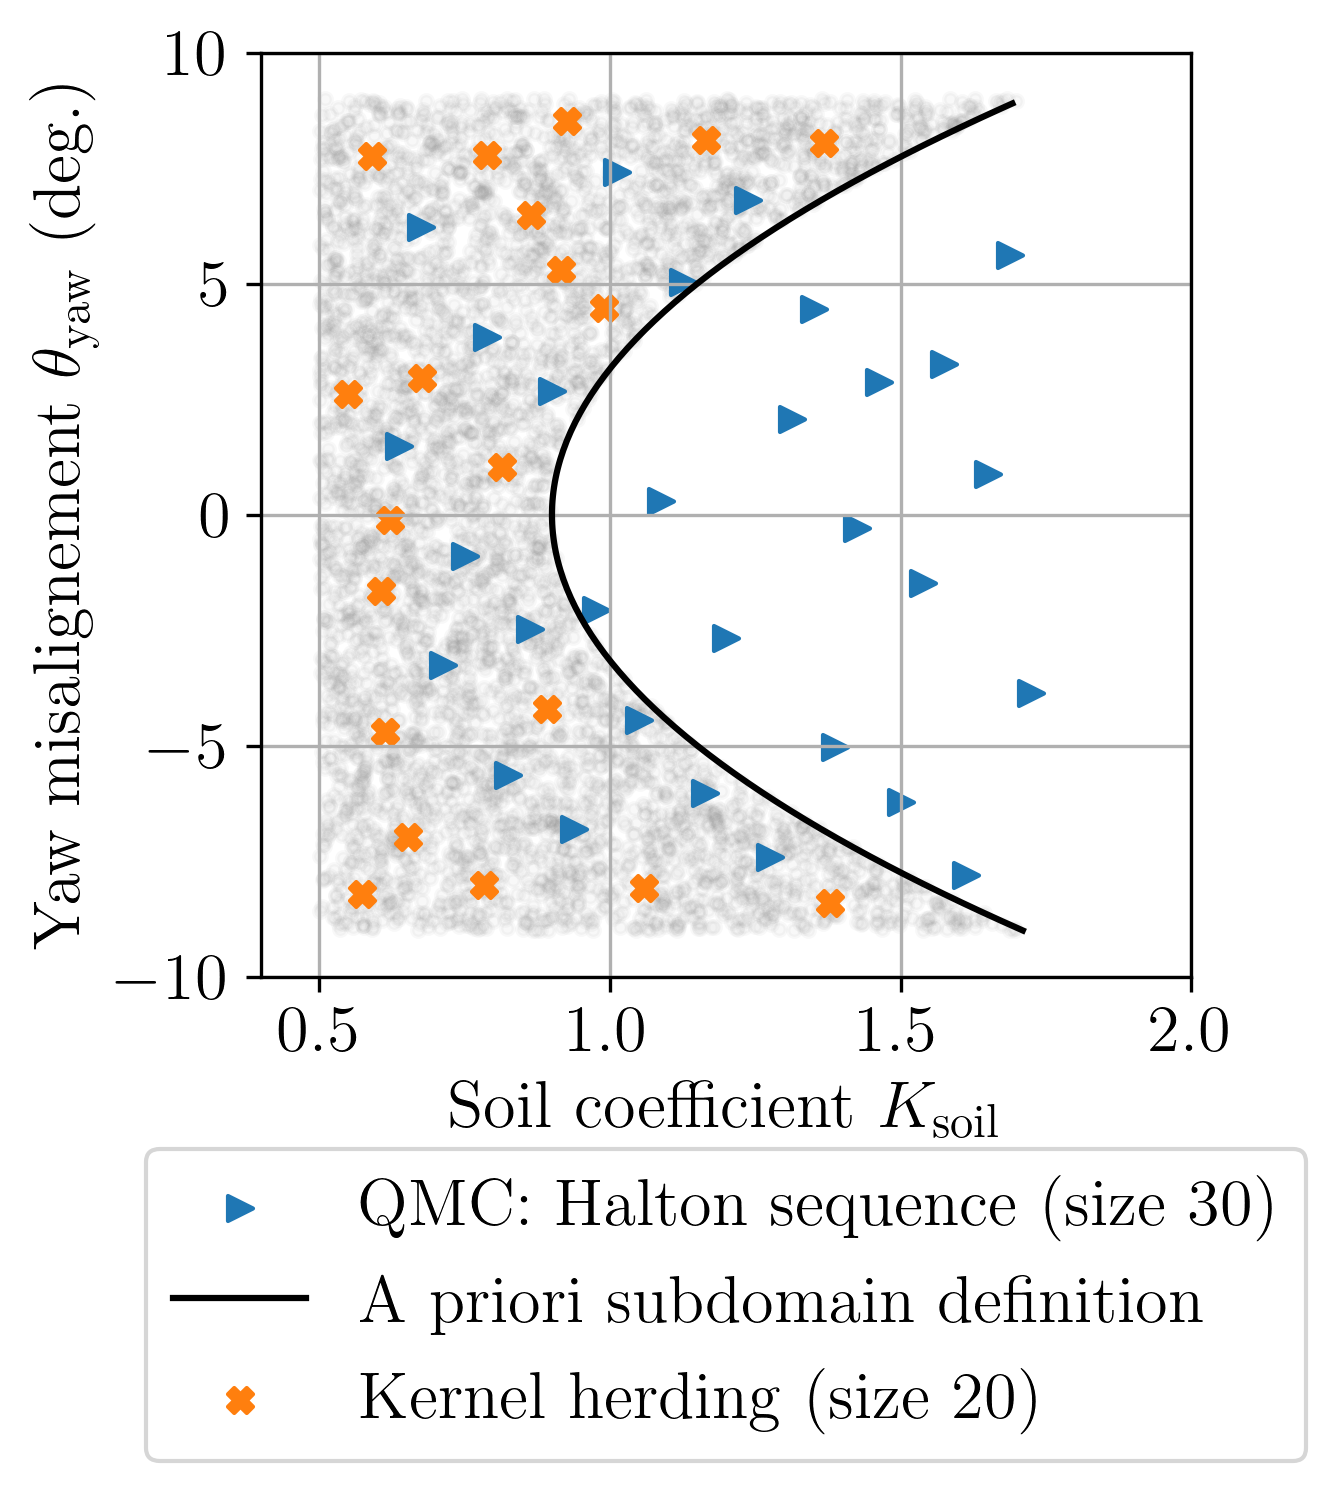
\includegraphics[width=\linewidth]{./part3/figures/OWT/initial_composite.png}
        \caption{Composite design.}
    \end{subfigure}
    \caption{Learning set of the mean damage surrogate model. A Halton sequence is first built (in blue) and completed by a set KH-generated points (in orange) in a subdomain defined a priori (in gray).}
    \label{fig:initial_doe}
\end{figure}

\begin{figure}[h!]
    \centering
    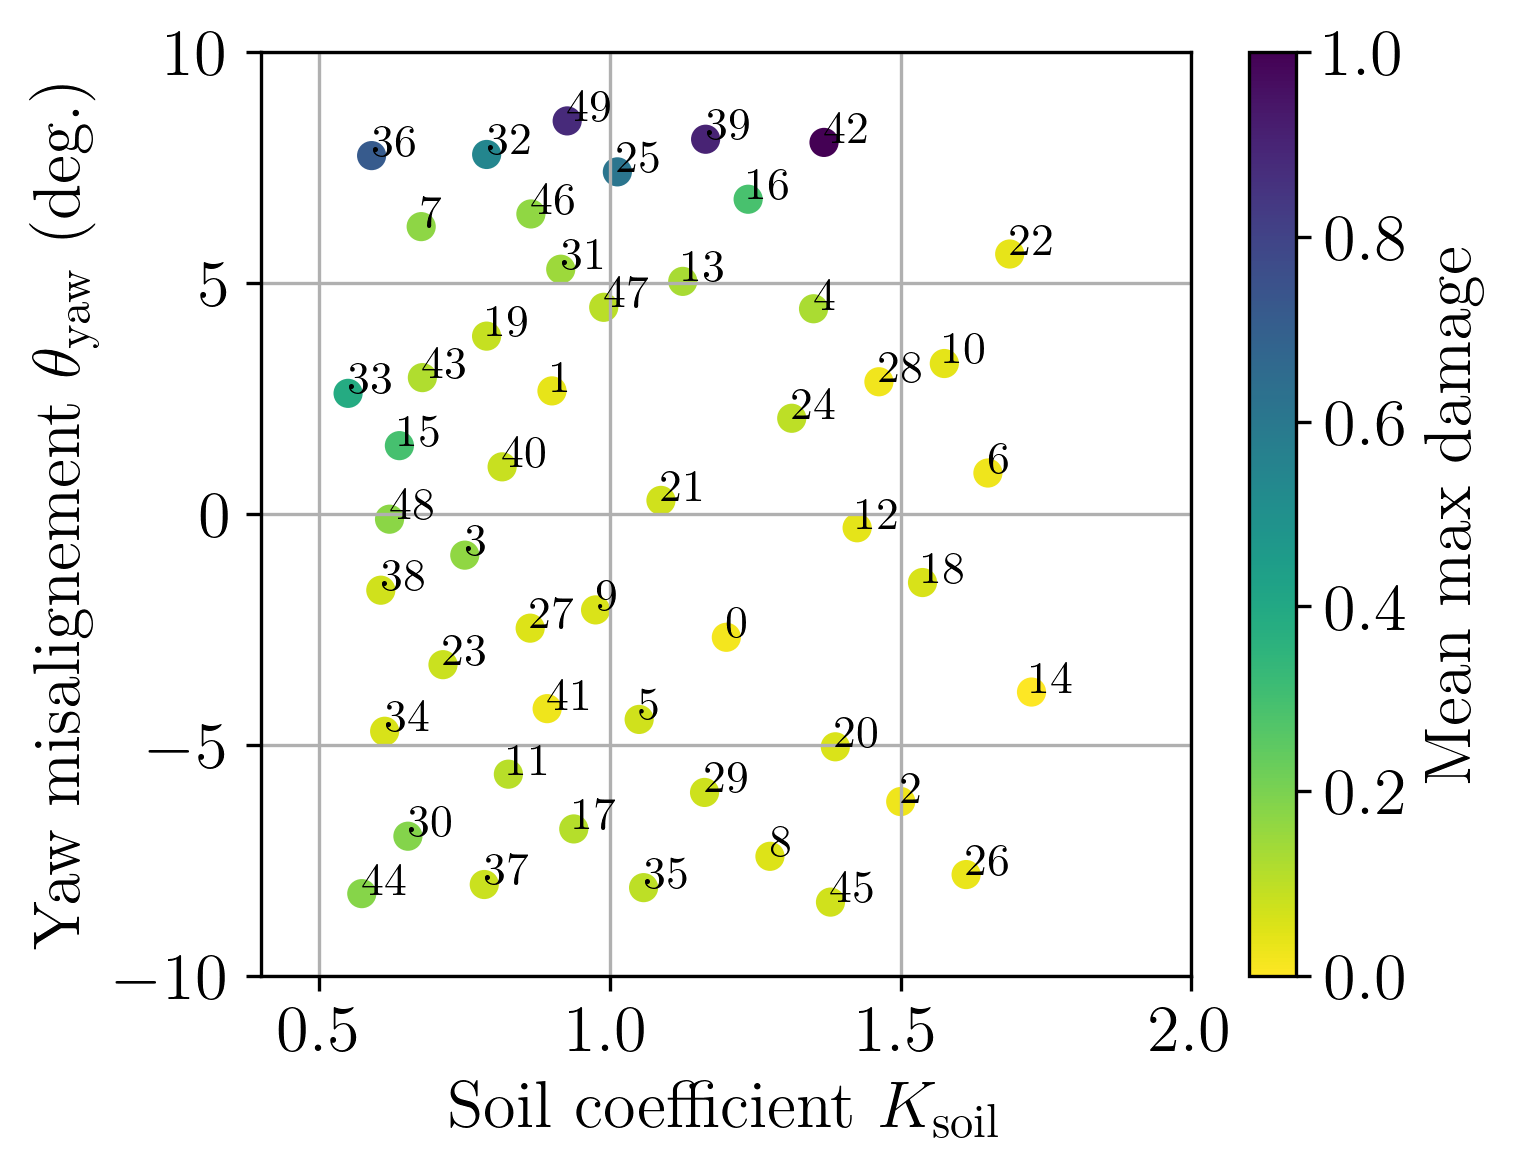
\includegraphics[width=0.6\linewidth]{./part3/figures/OWT/normalized_results_mean.png}
    \caption{Normalized mean damage evaluated on the mixed design illustrated in \fig{fig:initial_doe}.b.}
    \label{fig:evaluated_doe}
\end{figure}


%============================================================%
\subsection{Gaussian process regression}\label{sec:gp_owt}
%============================================================%
A GP regression with Matérn $5/2$ and constant trend is fitted on the mixed design $\bZ_{n_\bZ}$ according to the Kriging equations introduced in Section~\ref{sec:surrogate}. 
The resulting surrogate model $\widetilde{D}:\R^2 \rightarrow \R$, is represented by the blue three-dimensional surface in \fig{fig:3d_owt_surrogate}, and its learning set  $\bZ_{n_\bZ}$ by the black crosses.  
A complementary visualization of this surrogate is proposed for cross-sections with fixed values $\theta_{\mathrm{yaw}}=0$ on \fig{fig:owt_surrogate}.a, and $k_{\mathrm{soil}}=1$ on \fig{fig:owt_surrogate}.b. 
On these two figures, learning points are plotted in a grayscale and the surrogate model in a blue scale. 
The darker the shade, the closer to the cross-section the points are. 

One can first notice that the damage is not symmetric w.r.t. the yaw misalignment $\theta_{\mathrm{yaw}}$. 
When the nacelle perfectly aligns itself with the wind direction, this angle is equal to zero. 
For this bottom-fixed OWT, introducing a yaw error of the same amplitude has more impact in one direction than the other. 
In the meantime, the soil stiff $k_{\mathrm{soil}}$ has, as expected, a monotonic influence on the damage. 

To validate this surrogate model, a leave-one-out (LOO) procedure is realized. 
\fig{fig:loo_validation}.b represents the LOO squared-residuals at each point of the design (with values corresponding to the color scale). 
High residual values are mostly due to the strong nonlinearity of the code in some areas (as revealed by the cross-section in \fig{fig:owt_surrogate}.b).
\fig{fig:loo_validation}.a shows the quantile-quantile plot comparing the LOO predictions with the lifetime damage evaluations on the learning set. 
The general coefficient of predictivity of $\what{Q}^2_{\mathrm{LOO}}=0.72$ is considered acceptable in this small data context, especially as the LOO procedure was shown to underestimate the true performance metric in Chapter~\ref{chpt:5}. 
However, the surrogate could be enhanced by adding points to the learning set in areas with high nonlinearities.

\medskip
\begin{remark}
    Active learning methods for reliability assessment (see Subsection~\ref{sec:active_surrogates}) could be a great option for a such costly computer model. 
    However, the stochasticity of the function would disturb the learning criterion. 
    Since the nonlinearities seem restricted to a small area, the present approach should be more robust. 
    Another approach could be to fit a stochastic surrogate \citep{binois_2019_replication,baker_2022_stochastic_surrogates_review,zhu_2023_thesis} on a learning set before averaging on the pseudo-random seed repetitions.  
\end{remark}
\medskip

\begin{figure}[h!]
    \centering
    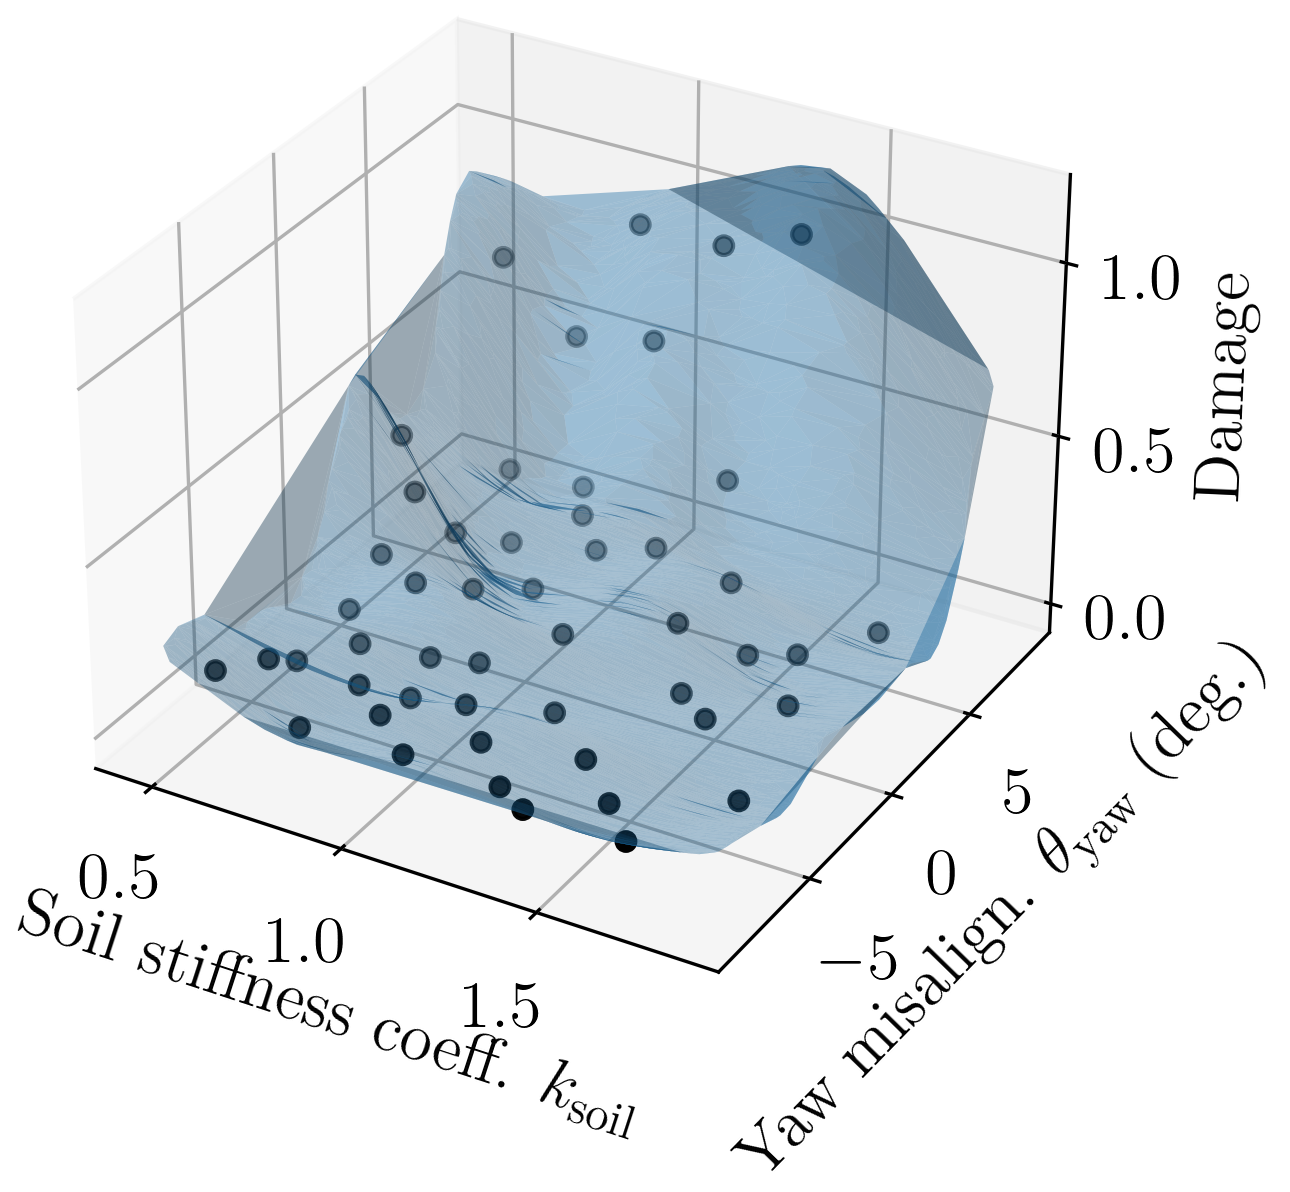
\includegraphics[width=0.45\linewidth]{./part3/figures/OWT/3D_surrogate.png}
    \caption{Three-dimensional plot of the surrogate model $\widetilde{D}$ (in blue) and learning set (in black).}
    \label{fig:3d_owt_surrogate}
\end{figure}

\begin{figure}[h!]
    \centering
    \begin{subfigure}[b]{0.38\linewidth}
        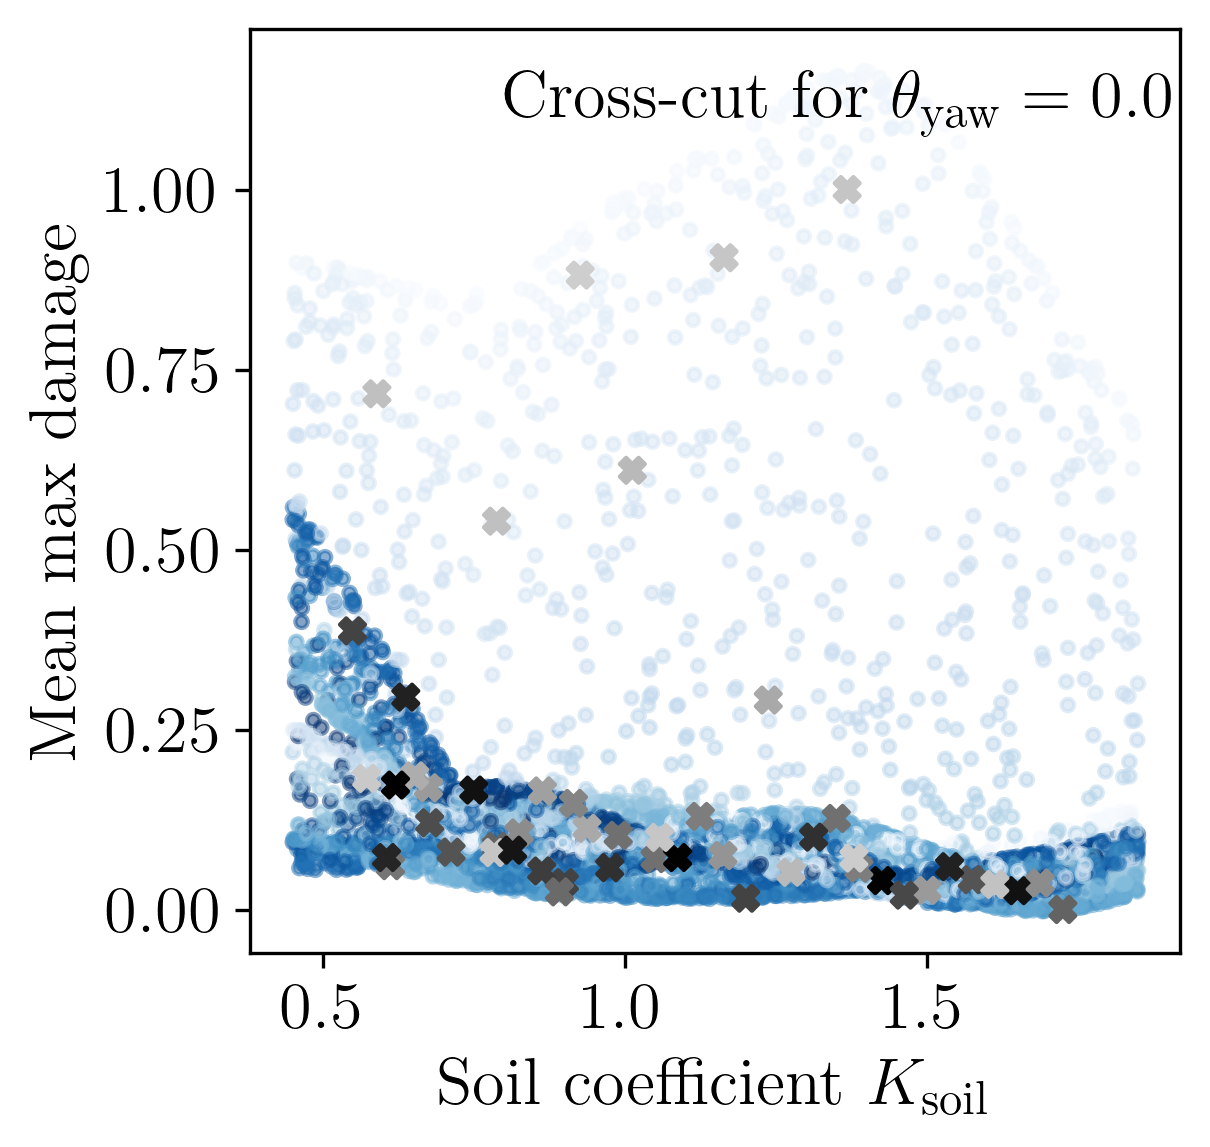
\includegraphics[width=\linewidth]{./part3/figures/OWT/dam_vs_soil_surrogate.png}
        \caption{$\theta_{\mathrm{yaw}}=0$.}
    \end{subfigure}
    \begin{subfigure}[b]{0.38\linewidth}
        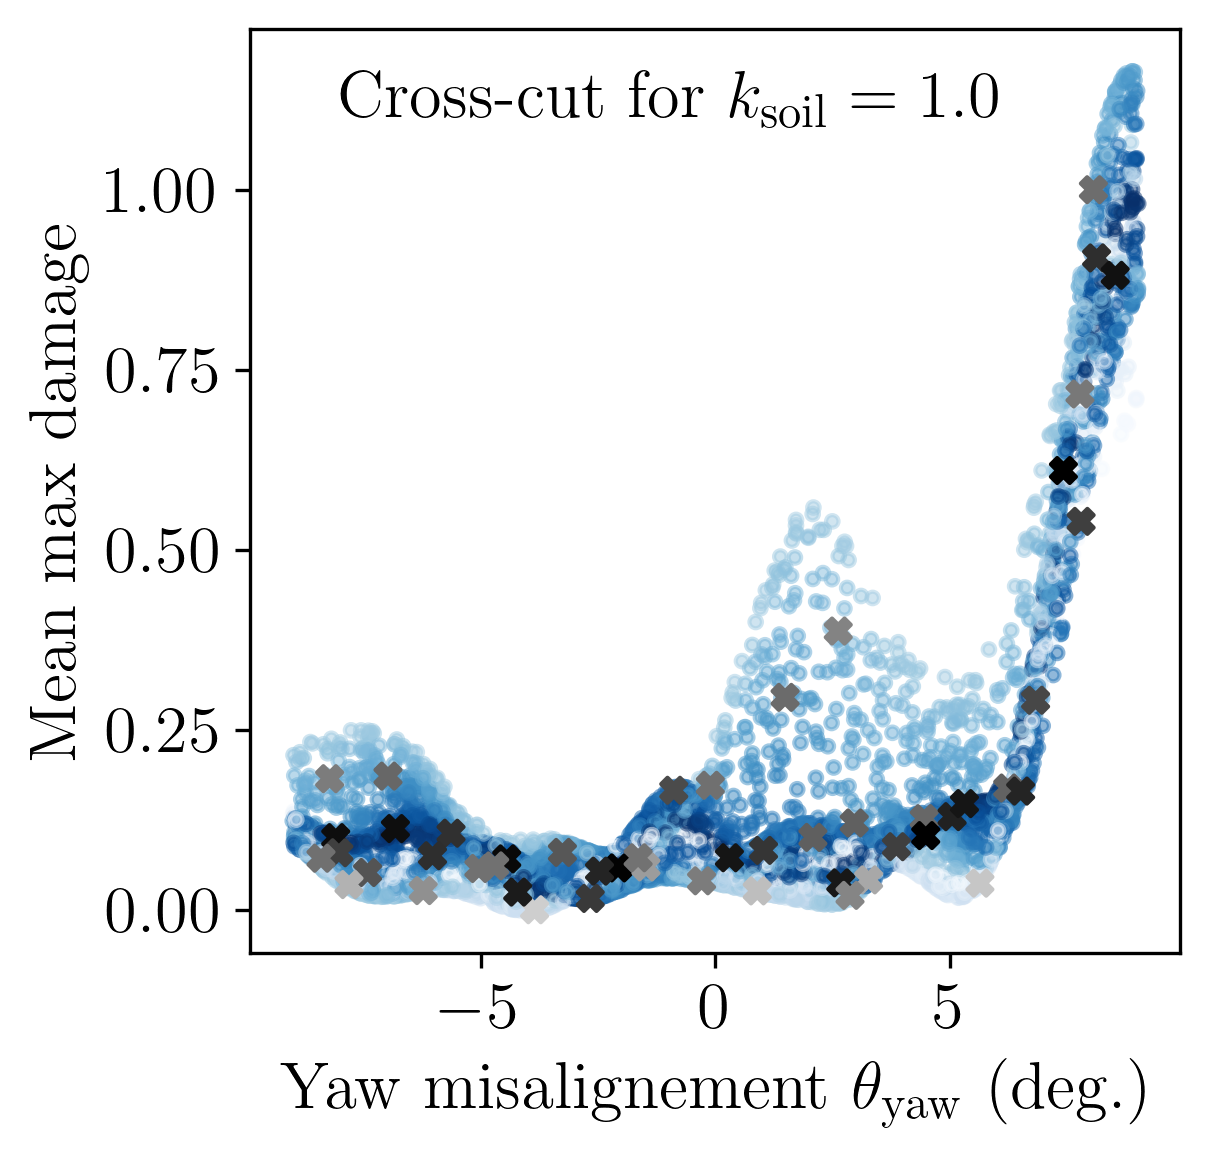
\includegraphics[width=\linewidth]{./part3/figures/OWT/dam_vs_yaw_surrogate.png}
        \caption{$k_{\mathrm{soil}}=1$.}
    \end{subfigure}
    \caption{Cross-section of the surrogate model $\widetilde{D}$ (in shades of blue) for given values of $K_{\mathrm{soil}}$ and $\Theta_{\mathrm{yaw}}$. The darker the shade, the closer to the cross-section.}
    \label{fig:owt_surrogate}
\end{figure}

\begin{figure}[h!]
    \centering
    \begin{subfigure}[t]{0.36\linewidth}
        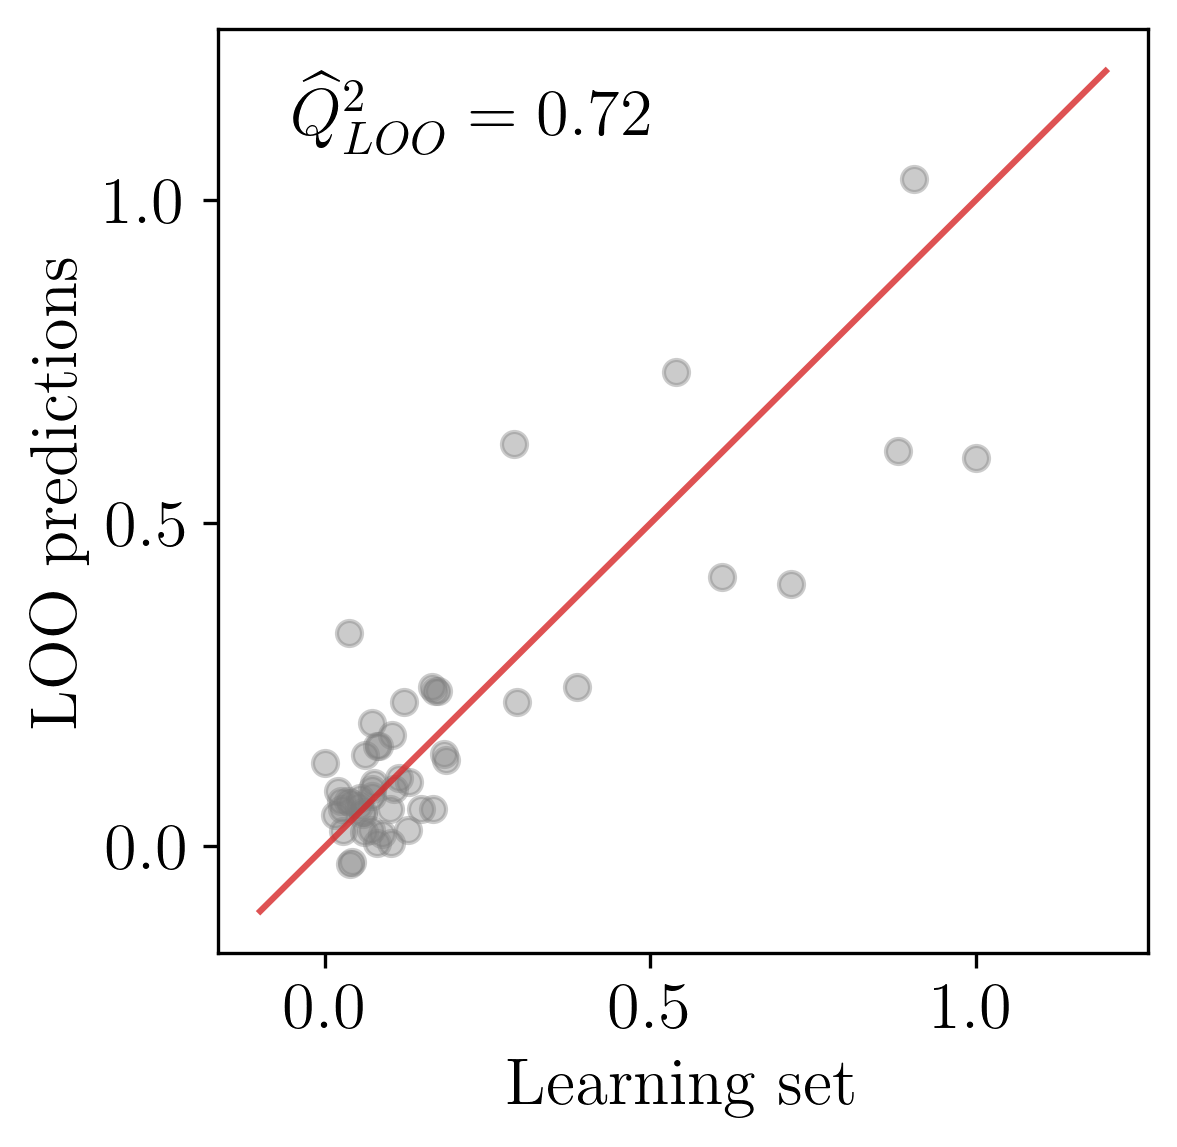
\includegraphics[width=\linewidth]{./part3/figures/OWT/loo_qqplot.png}
        \caption{Quantile-quantile plot.}
    \end{subfigure}
    \begin{subfigure}[t]{0.48\linewidth}
        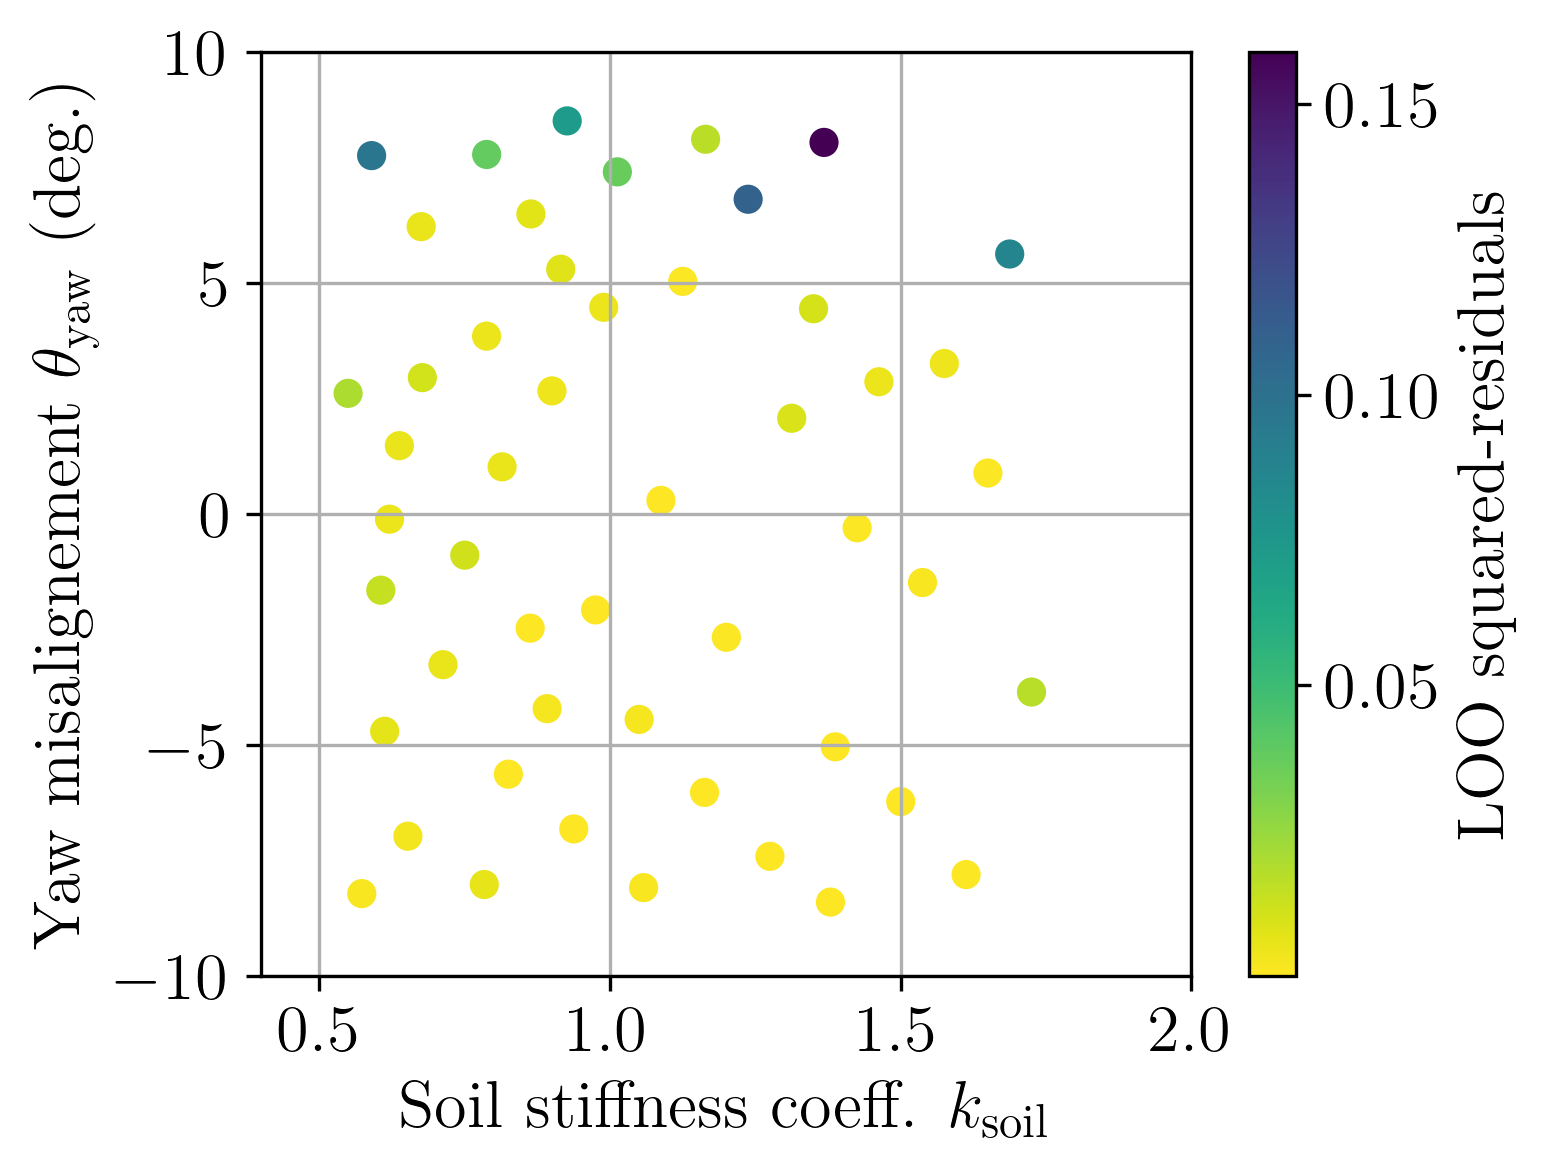
\includegraphics[width=\linewidth]{./part3/figures/OWT/loo_squared_res.png}
        \caption{LOO Squared-residuals.}
    \end{subfigure}
    \caption{Leave-one-out validation results of the surrogate model $\widetilde{D}$.}
    \label{fig:loo_validation}
\end{figure}

%============================================================%
%============================================================%
\section{Reliability and robustness analysis}
%============================================================%
%============================================================%
In the wind energy industry, acceptable risk levels for fatigue are defined by the standards. 
The target failure probability of the order of magnitude of $10^{-4}$ over the last year of exploitation is recommended by the \citet{iec_2019} while the recommendations of other standards are reviewed by \citet{wang_2022_owt_reliability_review}. 
\citet{nielsen_2021_risk_levels} discussed the relevance of this risk level, defined from an economic point of view, and offered quantitative guidelines for lifetime extension. 
In this section, a reliability analysis is conducted using the surrogate model of the lifetime cumulative damage previously constructed in Subsection~\ref{sec:gp_owt}. 
Afterwards, the robustness of this reliability analysis is studied by applying perturbations to the input distributions and computing the perturbed-law based sensitivity indices (PLI) initially proposed by \citet{lemaitre_2015_PLI}. 


%============================================================%
\subsection{Nominal reliability analysis}\label{sec:owt_ra}
%============================================================%
The S-N curve uncertainty can be expressed as a simple coefficient $\varepsilon$ (see Subsection~\ref{sec:probabilistic_sn}), which is applied to the lifetime cumulative damage as follows: 
\begin{equation}
    D(k_{\mathrm{soil}}, \theta_{\mathrm{yaw}}, \varepsilon) = \frac{1}{\varepsilon} \, D(k_{\mathrm{soil}}, \theta_{\mathrm{yaw}}, \varepsilon=1).
\end{equation}
Therefore, the surrogate model of the lifetime cumulative damage $\widetilde{D}$ is modified without updating its learning such as:
\begin{equation}
    \widetilde{D}'(\bz) = \widetilde{D}'(k_{\mathrm{soil}}, \theta_{\mathrm{yaw}}, \varepsilon) = \frac1\varepsilon \, \widetilde{D}(k_{\mathrm{soil}}, \theta_{\mathrm{yaw}}, \varepsilon=1).
\end{equation} 
The probability introduced in \eq{eq:owt_pf} then becomes: 
\begin{equation}
    \pf' = \int_{\iD_\bZ} \1_{\{\widetilde{D}'(\bz) \geq D_{\mathrm{cr}}\}} \, f_\bZ(\bz) \, \dd z.
    \label{eq:owt_pf_surrogate}
\end{equation}
Table~\ref{tab:pf_result_table} presents the estimates of this quantity by various methods (FORM, FORM-IS and SS, see Section~\ref{sec:reliability}) and for two different distributions of the resistance variable. 
$D_{\mathrm{cr}}$ either follows a lognormal distribution (which has a short left tail), or a normal distribution (with a heavier left tail). 
All methods deliver similar values of $\pf$ even if FORM-IS converges faster than SS when comparing the coefficients of variation (COV). 
The adequation of FORM with the simulation methods reveals that the LSF in this case is almost linear. 
This linearity is mostly due to the nature of the LSF, following a resistance-sollicitation paradigm as introduced earlier. 
%Such a conclusion might differ depending on the OWT model studied (e.g., a floating model could present a different behavior). 
The probabilities are, as expected, much lower under the hypothesis of lognormal distribution for $D_{\mathrm{cr}}$ than for a normal distribution. 
However, this significant difference questions the robustness of this result w.r.t. the probabilistic model of both $D_{\mathrm{cr}}$ and $\bZ$.  

\begin{table*}[h]
    \centering
    \caption{Nominal reliability analysis (size $N=5 \times 10^4$ for IS and SS. $p_0=0.1$ for SS).}
    \begin{tabular}{r||c|c|c|c}
              &  \multicolumn{2}{c|}{$D_{\mathrm{cr}} \sim $ \bf Lognormal} & \multicolumn{2}{c}{$D_{\mathrm{cr}} \sim $ \bf Normal}\\
    \hline
    \bf Reliability method & $\widehat{\pf}'$       & $\widehat{\mathrm{cov}}$    & $\widehat{\pf}'$       & $\widehat{\mathrm{cov}}$ \\
    \hline\hline
    FORM      & $9.87 \times 10^{-13}$ & --                    & $3.35 \times 10^{-6}$ & --\\
    \hline
    FORM-IS   & $9.84 \times 10^{-13}$ & $1 \%$                & $3.36 \times 10^{-6}$ & $1 \%$\\
    \hline
    SS        & $9.46 \times 10^{-13}$ & $7 \%$               & $3.50 \times 10^{-6}$ & $4 \%$\\ 
    \end{tabular}
    \label{tab:pf_result_table}
\end{table*}


%============================================================%
\subsection{Robustness analysis using perturbed-law sensitivity indices}\label{sec:owt_robustness}
%============================================================%
The method of \citet{lemaitre_2015_PLI}, later called \textit{perturbed-law based sensitivity indices} (PLI) by \citet{sueur_2017_PLI} relies on perturbating input densities. 
The goal is to assess the robustness of a quantity of interest (here, a failure probability) w.r.t. these perturbations. 
This type of index is for example used in studies of thermal-hydraulic numerical models for nuclear safety \citep{iooss_2022_pli}. 
%\elias{Place the PLI in the robustness litterature?}

Assuming a random variable $Z_j \sim f_j \in \iD_{Z_j}$ with mean $\E[Z_j]=\mu$ and variance $\var(Z_j) = \sigma^2$, the strategy is to find the ``closest'' distribution $f_{j \delta}$ under the constraint of moment perturbation of magnitude $\delta$.  
The notion of proximity between distributions is quantified by \citet{lemaitre_2015_PLI} in terms of Kullback–Leibler (KL) divergence. 
For example, a relative mean perturbation is defined as: 
\begin{eqnarray}
    f_{j \delta} = \argmin_{\substack{\pi\in \mathcal{P}, \\ \mathrm{s.t.}, \E_\pi[Z_j] = \E_{f_j}[Z_j](1 + \delta)}} \, \mathrm{KL}(\pi||f_j)\, , 
\end{eqnarray} 
where $\delta \in \R$ denotes the relative perturbation, and $\mathcal{P}$ is a family of distributions. 

Note that the perturbed distribution $f_{j \delta}$ might not belong to the parametric family of $f_j$. 
This is typically the case for bounded distributions (e.g., when perturbating the mean of a uniform distribution). 
Separate approaches exist to define perturbations for the problem studied, such as \citet{lemaitre_2015_PLI}, or \citet{gauchy_2022_PLI}. 
However, to ease the computation in the following, the perturbations will conserve the initial parametric family (which seems reasonable for distributions in the exponential family). 

The adapted expression of the PLI used hereafter \citep{gauchy_2022_PLI} reflects the relative impact of a perturbation on the quantity of interest: 
\begin{equation}
    \mathrm{PLI}\left(f_{j \delta}\right) = \frac{p_{\mathrm{f}, j \delta} - \pf }{\pf} \,,
\end{equation}
where $p_{\mathrm{f}, j \delta}$ is the probability obtained when injecting $f_{j \delta}$ in \eq{eq:owt_pf_surrogate}.
In the following, each variable in $\bZ$ is perturbed one by one in terms of relative standard deviation, such that $\sigma_{j \delta} = \sigma_j (1+\delta)$. 
The illustration of such perturbations is illustrated in \fig{fig:perturbations}, for distributions of $K_{\mathrm{soil}}$ on the left, and of $\Theta_{\mathrm{yaw}}$ on the right.
This strategy assumes that the analyst has enough information to determine the mean of the variables $Z_j$. 

The resulting PLI are presented in \fig{fig:pli_all} for relative perturbations of the standard deviations of $(K_{\mathrm{soil}}, \Theta_{\mathrm{yaw}}, \varepsilon)$. 
Each failure probability is independently estimated by FORM-IS. 
In the hypothesis of a normal $D_{\mathrm{cr}}$, the most important variable is $\Theta_{\mathrm{yaw}}$, while the fluctuations are quite stable in the hypothesis of a lognormal $D_{\mathrm{cr}}$. 

When perturbating the standard deviation of the resistance variable $D_{\mathrm{cr}}$, the same phenomenon is witnessed in \fig{fig:pli_resistance}. 
The perturbations have nearly no consequences, assuming that $D_{\mathrm{cr}}\sim \mathrm{LogNormal}$, but a lot of influence when $D_{\mathrm{cr}}\sim \mathrm{Normal}$.  
As a perspective, this study could be completed by a joint perturbation of both the standard deviation and mean of the resistance variable.


\begin{figure}
    \centering
        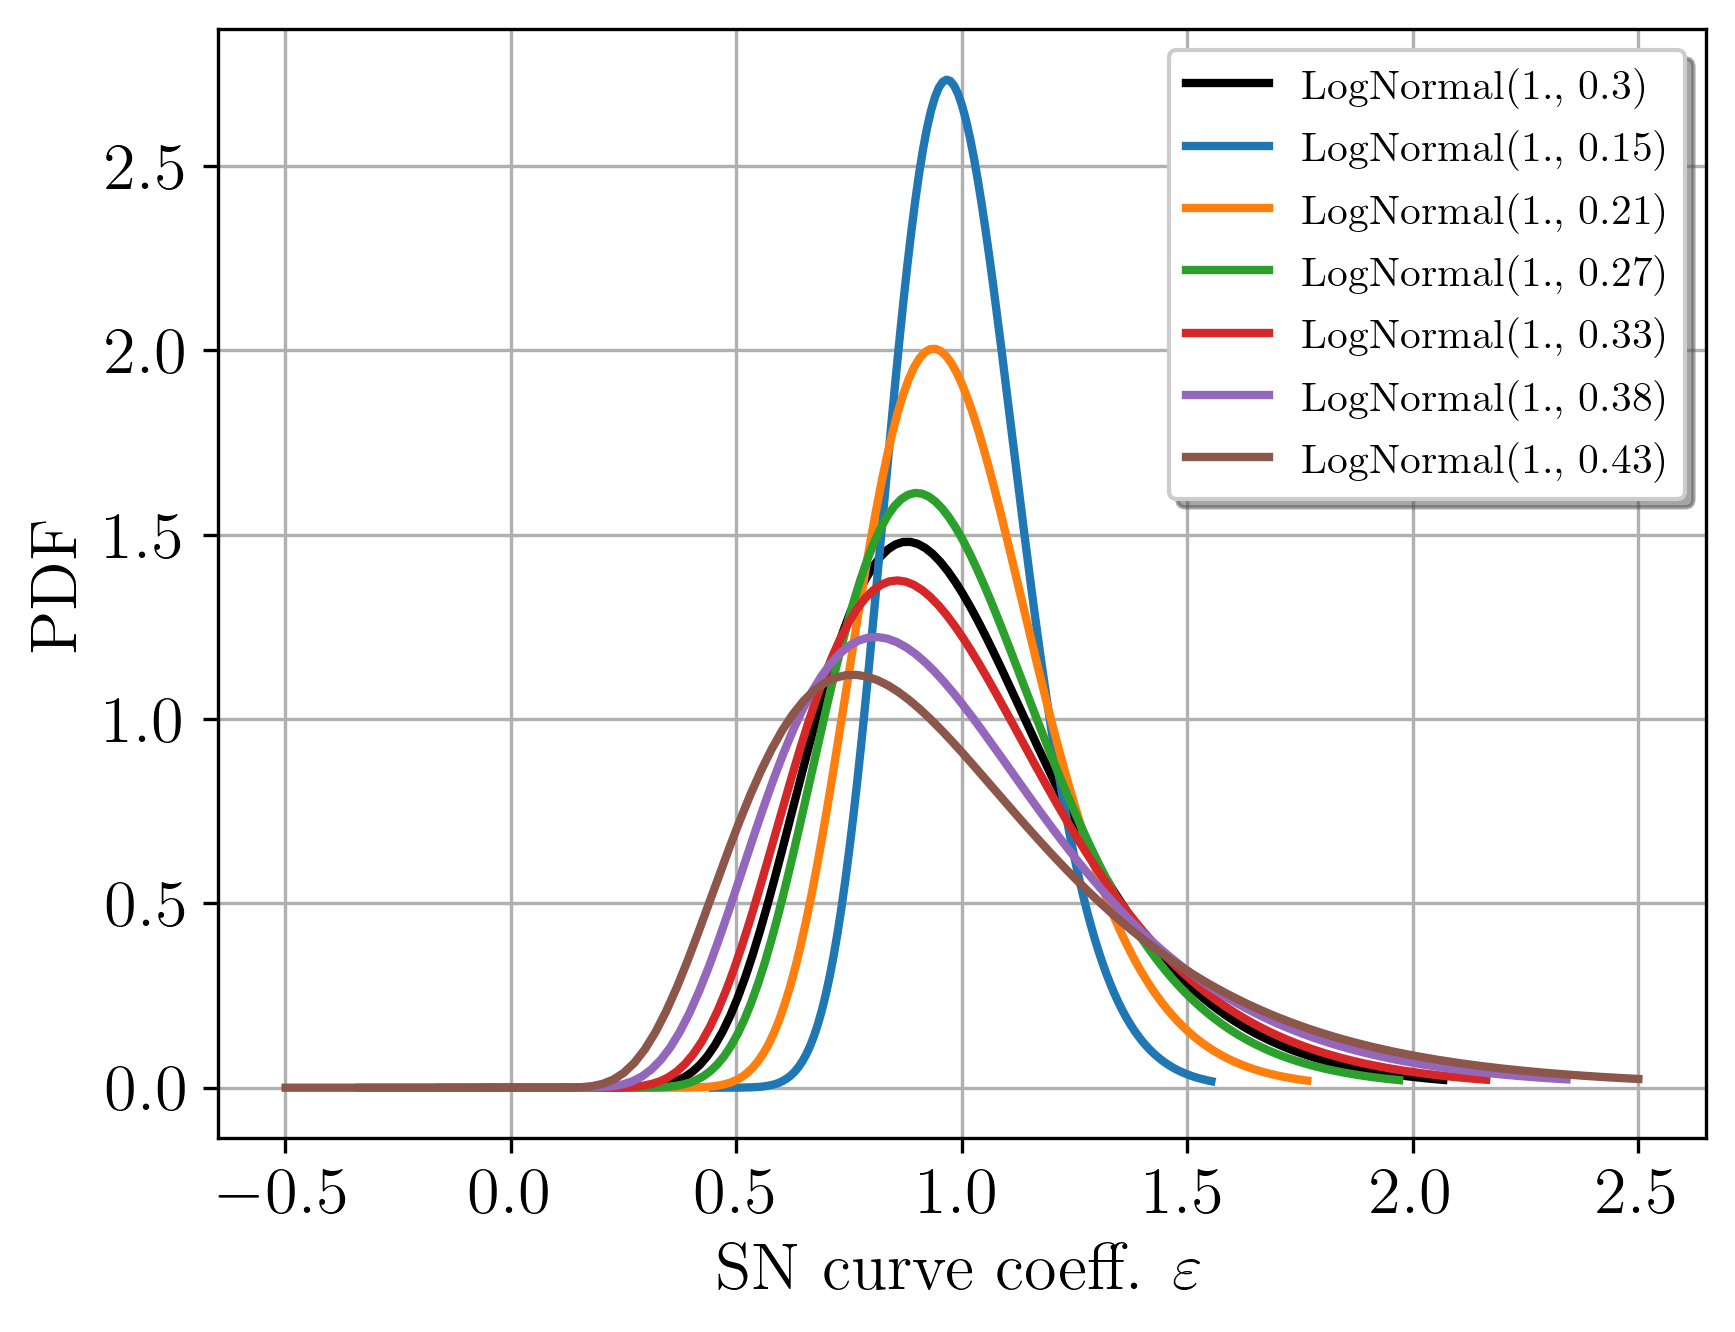
\includegraphics[width=0.43\linewidth]{./part3/figures/OWT/lognormal_pert.png}
        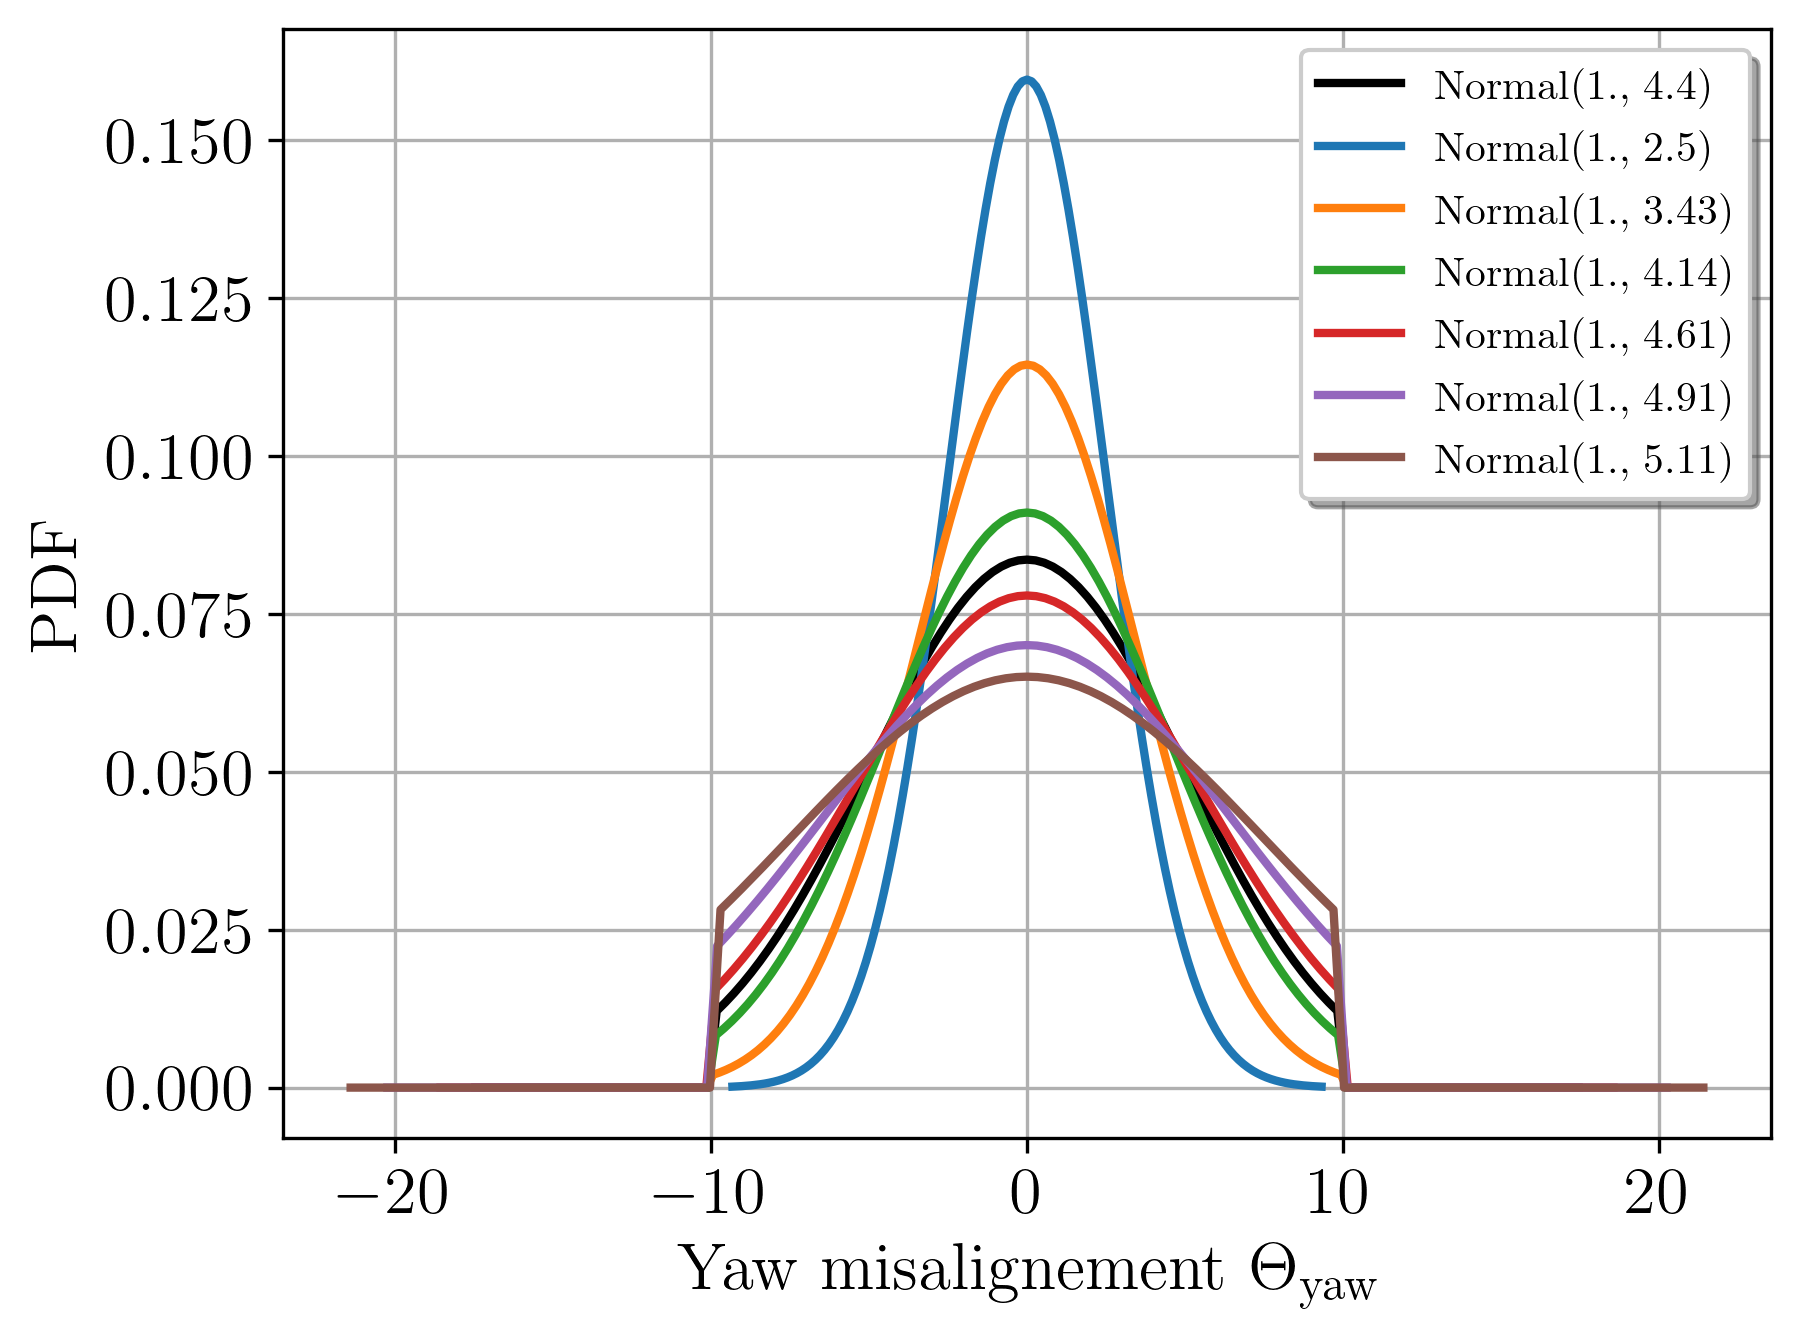
\includegraphics[width=0.44\linewidth]{./part3/figures/OWT/normal_pert.png}
    \caption{Perturbations in terms of standard deviation of a lognormal distribution (left) and a truncated normal distribution (right).}
    \label{fig:perturbations}
\end{figure}


\begin{figure}
    \centering
    \begin{subfigure}[t]{0.48\linewidth}
        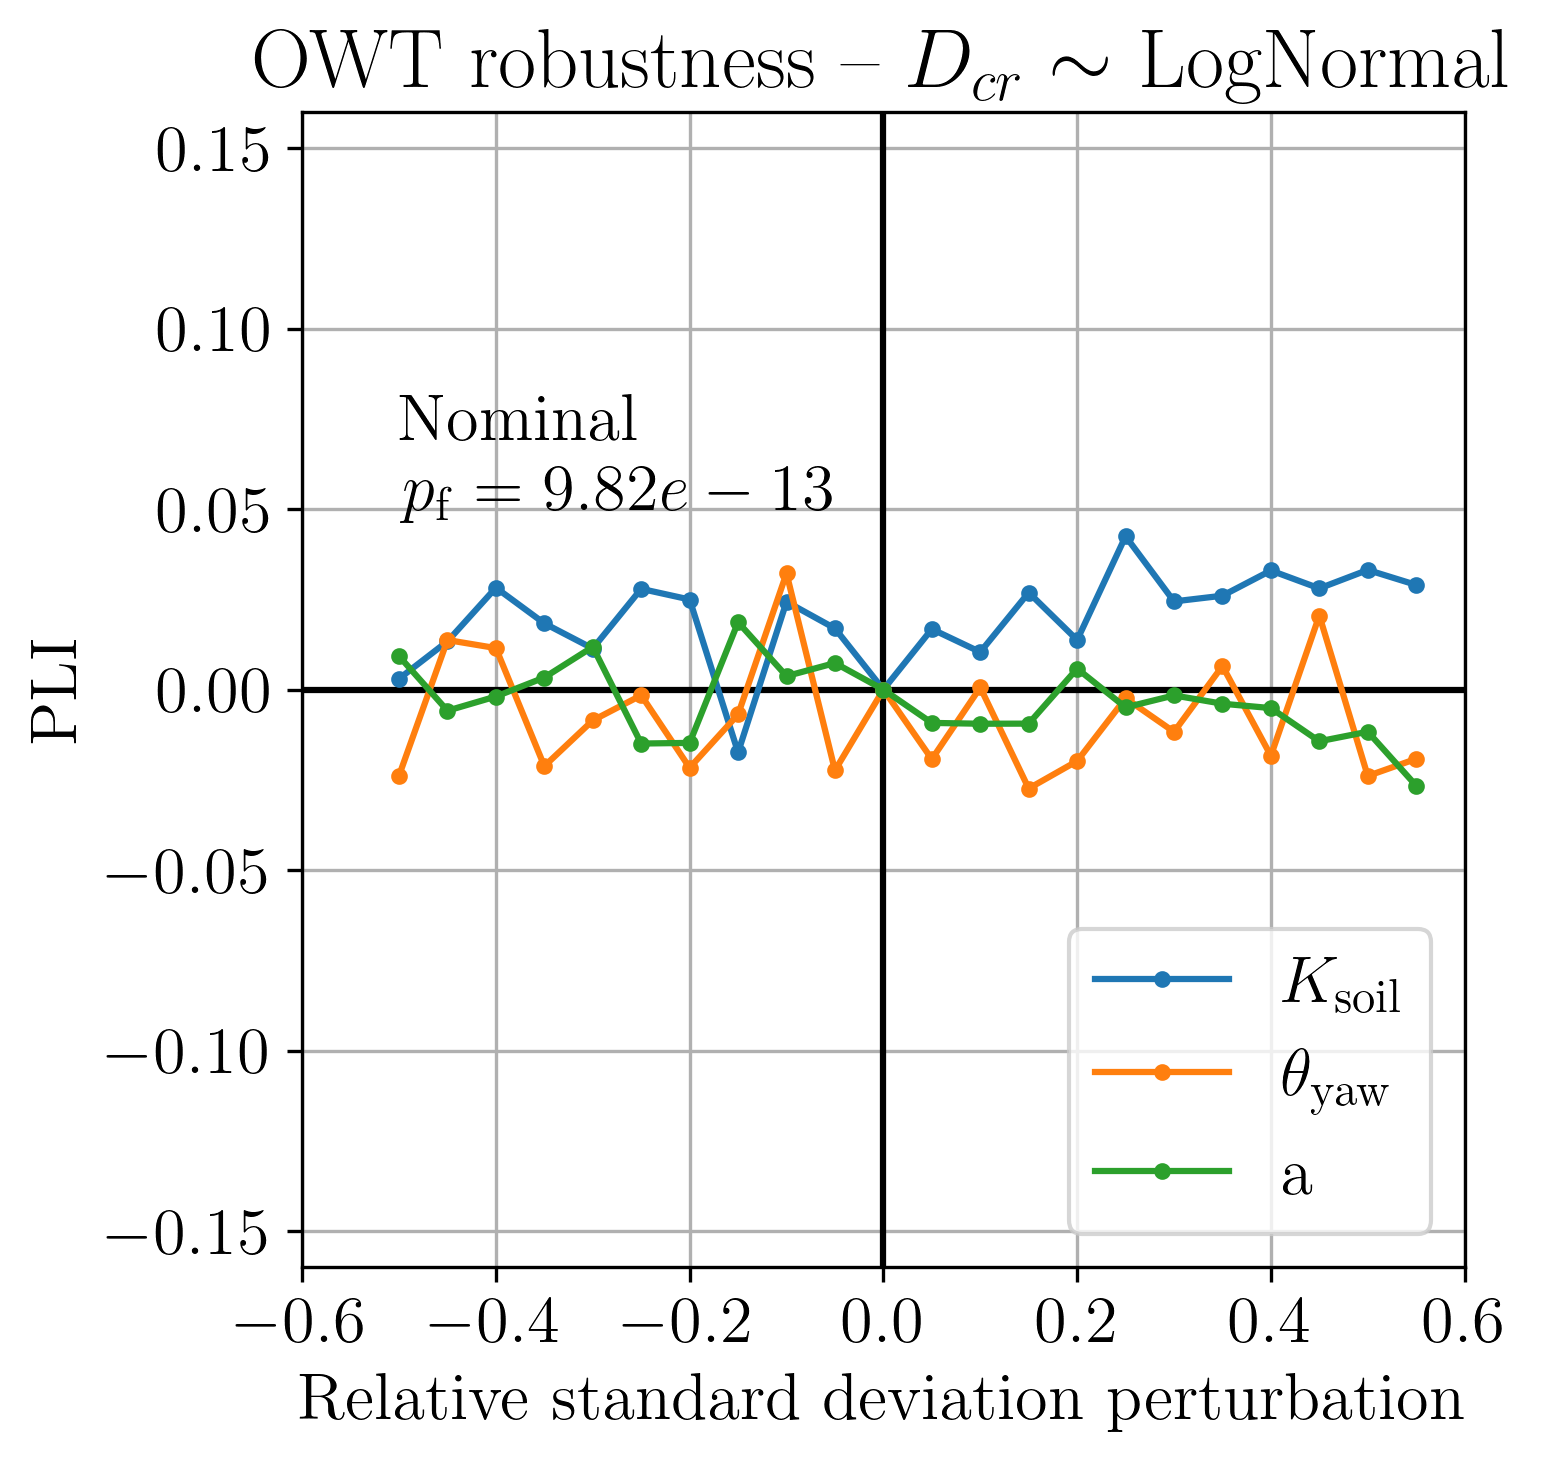
\includegraphics[width=\linewidth]{./part3/figures/OWT/PLI_ALL_Hyp_LogNormal.png}
        \caption{$D_{\mathrm{cr}} \sim $ Lognormal.}
    \end{subfigure}
    \begin{subfigure}[t]{0.48\linewidth}
        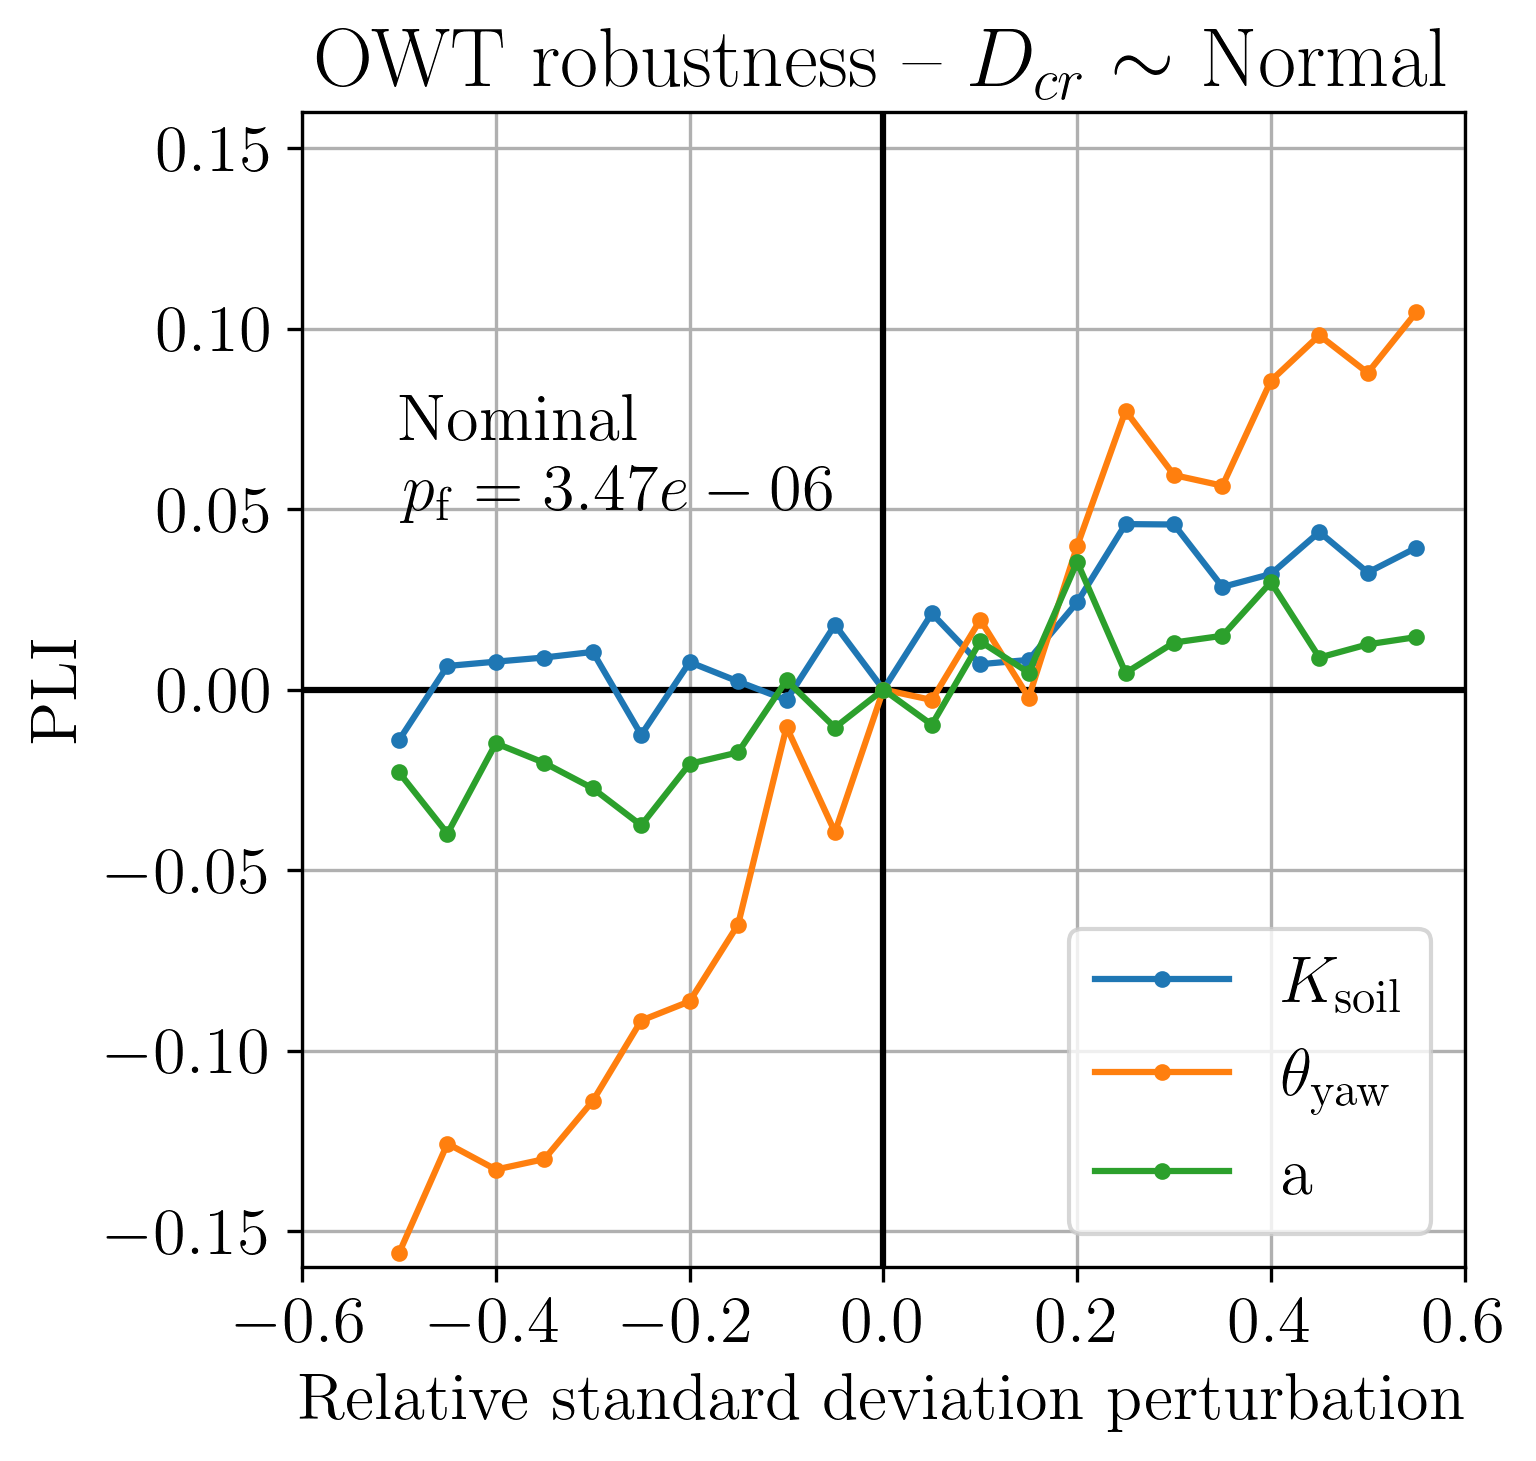
\includegraphics[width=\linewidth]{./part3/figures/OWT/PLI_ALL_Hyp_Normal.png}
        \caption{$D_{\mathrm{cr}} \sim $ Normal.}
    \end{subfigure}
    \caption{Perturbed-law based indices for relative perturbations of the standard deviations of $(K_{\mathrm{soil}}, \Theta_{\mathrm{yaw}}, \varepsilon)$. 
    The failure probabilities studied are each estimated by FORM-IS method with sample size $N=5 \times 10^4$.}
    \label{fig:pli_all}
\end{figure}


\begin{figure}
    \centering
    \begin{subfigure}[t]{0.48\linewidth}
        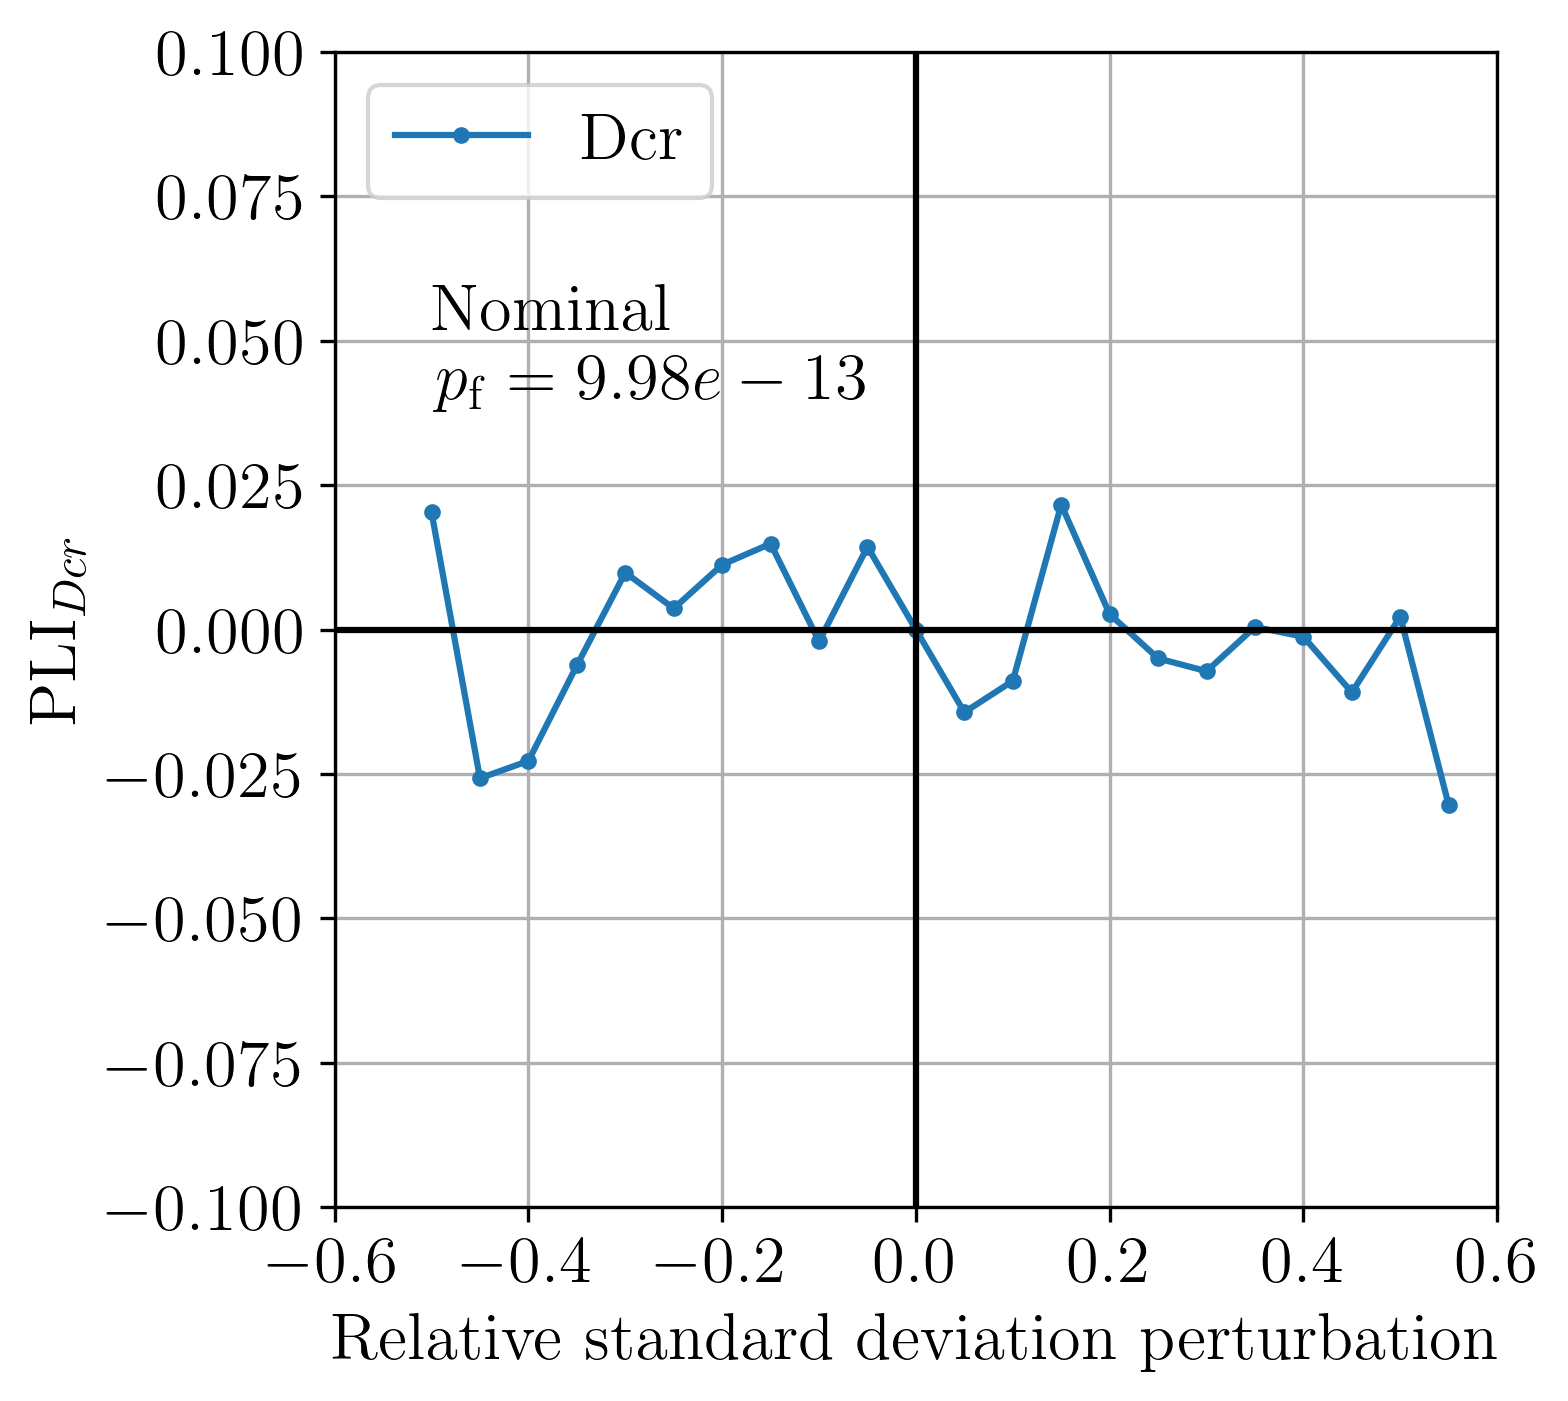
\includegraphics[width=\linewidth]{./part3/figures/OWT/PLI_Dcr_Hyp_LogNormal.png}
        \caption{$D_{\mathrm{cr}} \sim $ Lognormal.}
    \end{subfigure}
    \begin{subfigure}[t]{0.45\linewidth}
        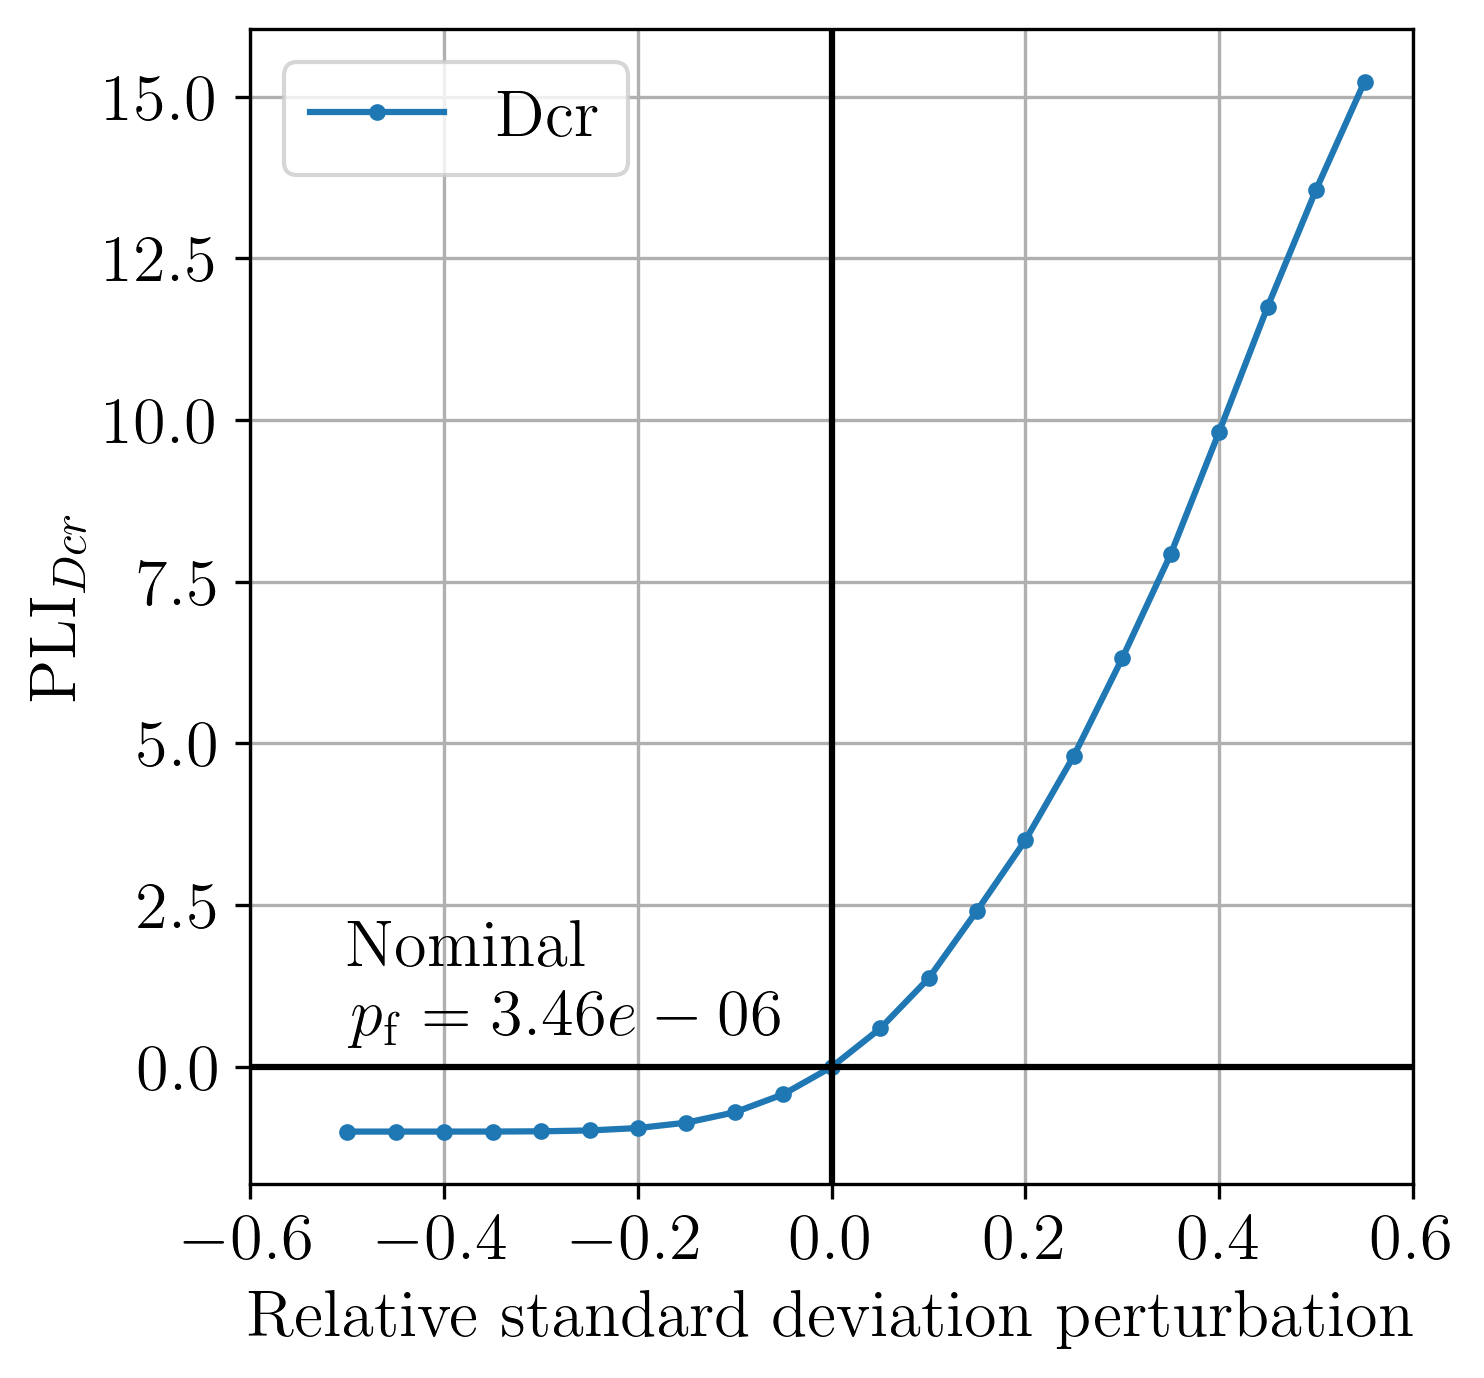
\includegraphics[width=\linewidth]{./part3/figures/OWT/PLI_Dcr_Hyp_Normal.png}
        \caption{$D_{\mathrm{cr}} \sim $ Normal.}
    \end{subfigure}
    \caption{Perturbed-law based indices for relative perturbations of the standard deviation of $D_{\mathrm{cr}}$. 
    The failure probabilities studied are each estimated by FORM-IS method with sample size $N=5 \times 10^4$.}
    \label{fig:pli_resistance}
\end{figure}

\newpage
%============================================================%
%============================================================%
\section{Conclusion}
%============================================================%
%============================================================%

In this chapter, a fully probabilistic reliability analysis was performed on the monopile foundation of an OWT located in Teesside, UK. 
This first reliability study required a significant computational effort (i.e., over $10^5$ Turbsim-DIEGO simulations), made possible with the development of a tailored wrapper deployed on a HPC facility. 
These simulations served the construction of a surrogate model emulating the lifetime damage function. 

The second section of this chapter addressed the estimation of a failure probability using this surrogate model. 
A general conclusion is that this probability is highly dependent on the probabilistic model describing the critical damage. 
To challenge the modeling assumptions of the critical damage and the system variables, a robustness analysis was realized. 
It consists in studying the impact of perturbating the input distributions on an output quantity.   
The robustness of the failure probability was evaluated with the formalism of the perturbed-law based indices, introduced by \citet{lemaitre_2015_PLI}.
This additional study mostly confirmed the importance of the critical damage definition. 

From an industrial point of view, the failure probabilities obtained are lower than the risk levels targeted in current standards \citep{wang_2022_owt_reliability_review}, which is in favor of lifetime extension. 
However, the results of this demonstrative study may be questionable with respect to several assumptions that have been made: 
\begin{itemize}
    \item The periods in parked position which could significantly increase the damage (see \citealp{velarde_2020_fatigue_reliability}). 
    Several studies showed that the aerodynamic damping created by the rotation of the turbine reduces tower vibrations, and therefore fatigue \citep{liu_2017_damping};
    \item The rapid transition phases occasioned by emergency stopping, which might increase fatigue;
    \item The early damage produced during the installation of the monopile foundations by hydraulic impact piling (i.e., hammering);  
    \item The stress-concentration resulting from soldering the structure.
\end{itemize} 
An interesting industrial perspective could be to reproduce a similar study on a floating OWT model and compare the conclusions drawn from both studies.  

As a final perspective, a stochastic surrogate model could be built by considering all the damages without averaging them over the environmental repetitions. 
The risk assessment would then be conducted on a stochastic function. 
In this particular context, quantile estimation was studied by \cite{browne_2016_stochastic_quantile}, however, rare event estimation on stochastic functions remains an open question recently discussed by \citet{pires_2023_noisy_RA}. 
